% EPL master thesis covers template
\documentclass{EPL-master-thesis-covers-EN}

%% Includes

%Acronyms
\usepackage[acronym]{glossaries}

%Format
\usepackage{parskip}
\newcommand{\forceindent}{\parindent=1em\indent\parindent=0pt\relax}
%%Images
\usepackage{graphicx}
\usepackage{pgf}
\usepackage{caption}
\usepackage{subcaption}
\usepackage{float}

%%Minted for code
\usepackage{minted}
\setminted[text]{breaklines, autogobble}
\usemintedstyle{borland}
\setminted[erlang]{breaklines, autogobble}

%% Math
\usepackage{amsmath}
\usepackage{amssymb}
\usepackage{relsize}
\usepackage{dsfont}
\usepackage{bigints}

\usepackage{listings}
\usepackage{accents}
\usepackage{hyperref}
%Appendix
\usepackage[toc,page]{appendix}

%Bibliography

\usepackage[
backend=biber,
style=numeric,
sorting=none
]{biblatex}

\addbibresource{biblio.bib}


% Please fill in the following boxes
% What if I didn't?
% Title of the thesis
\title{Observing the detailed behaviour of large distributed applications in real time using $\Delta$QSD}

% Name of the student author(s)
\author{Francesco \textsc{Nieri}}
\degreetitle{Master [120] in Computer Science}

% Name of the supervisor(s)
\supervisor{Peter \textsc{Van Roy}}

% Name of the reader(s)
\readerone{Tom \textsc{Barbette}}
\readertwo{Peer \textsc{Stritzinger}}			% remove if not applicable
\readerthree{Neil \textsc{Davies}}			% remove if not applicable

% Academic year (update if necessary)
\years{2024--2025}

% Document
\begin{document}
  % Front cover page
    \maketitle
   
    \renewcommand{\thepage}{\roman{page}}

    \newgeometry{left=3cm, right=2.5cm, top=3cm, bottom=3cm} % Adjust as needed
    \chapter*{Abstract}
    It is difficult to study the detailed behaviour of large distributed systems while they are running. Many important questions are hard to answer. What happens when there is an overload? How can we feel something is wrong with the system early enough?

    The purpose of the thesis is to create the $\Delta$Q oscilloscope, a real time graphical dashboard that can be used to study the behaviour of running Erlang systems and explore tradeoffs in system design. It is based on the principles of $\Delta$QSD.
  
    Furthermore, we have developed an Erlang interface, the $\Delta$Q adapter (\texttt{dqsd\_otel}). It allows sending real time insights about the running system to the oscilloscope. The adapter works on top of the OpenTelemetry framework macros. This allows for users who have already instrumented their applications with OpenTelemetry to integrate the interface for the oscilloscope.
    
    The oscilloscope performs statistical computations on the time series data it receives from the adapter and displays the results in real time, thanks to the $\Delta$QSD paradigm. We provide a set of triggers to capture rare events, like an oscilloscope would, and give a snapshot of the system under observation, as if it was frozen in time. An implementation of a textual syntax allows the creation of outcome diagrams which give an ``observational view'' of the system. Furthermore, the implementation of efficient algorithms for complex operations, such as convolution, allows for the computations to be done rapidly on precise representations of components.

    We introduce the work by giving a summary of $\Delta$QSD concepts. We also provide a summary of the observability tools available for Erlang, namely, OpenTelemetry. We then present the overall design of the project, describing how to build a bridge from OpenTelemetry to the oscilloscope. Subsequently, we explain the user level concepts which are essential to understand how the oscilloscope works and understand what is displayed on the screen, delving later on into the mathematical foundations of the concepts. Lastly, we provide synthetic applications which prove the soundness of $\Delta$QSD and show how the oscilloscope is able to detect problems in a running system, diagnose it and explore design tradeoffs.




    \chapter*{Acknowledgments}
    This thesis is the culmination of my studies, I would like to thank the people who made this possible, those who supported me through the years and those who helped my with the thesis.
    
    \forceindent My family, especially \textbf{my mom, my dad, my brother} and \textbf{my sister}, for their help which was a crucial shoulder I could lay on while writing this thesis and most importantly throughout these five years.
    
    \forceindent My \textbf{friends}, to those who have taken time out of their lives to listen the thesis presentation and to those who through the years have been there for me. 

    \forceindent \textbf{A-M.}, for the moments we shared these four years together in uni.

    \forceindent \textbf{My dad} and \textbf{Maurizio}, who nurtured the passion for coding in me.
    
    \forceindent \textbf{Peer Stritzinger}, \textbf{Stritzinger GmbH} and the \textbf{EEF Observability Working Group} (Bryan Naegele and Tristan Sloughter) for their help in the EEF Slack, which helped me in understanding OpenTelemetry and gave me the send\_after intuition.

    \forceindent \textbf{Neil Davies} for taking the time to proofread my thesis.

    \forceindent The \textbf{PNSol Ltd.} team for their extensive groundwork on \textbf{$\Delta$QSD} and its dissemination, which made this thesis possible.

    \forceindent Lastly, \textbf{Peter Van Roy}, for his year-long relentless interest, support and weekly and constant supervision which made sure the project would come to fruition. 


    \chapter*{AI disclaimer}
    AI was used to help writing the dashboard interface and to help with the Erlang side.

    The written master thesis was written entirely without the aid of AI.

    \tableofcontents 

    \cleardoublepage
 
    \printglossary[type=\acronymtype,style=long]
    \pagenumbering{arabic}% Reset page numbering and style
    
    \chapter{Introduction}
     \section{Approach}
    In the context of this thesis, the \textbf{$\Delta$QSD paradigm} has been used to develop a tool to study the real-time behaviour of running systems. \\
    As described by a tutorial given on $\Delta$QSD \cite{dq-tut}:
    \begin{quote}
        ``$\Delta$QSD is an industrial-strength approach for large-scale system design that can predict performance and feasibility early on in the design process.'' 
    \end{quote}
    The paradigm has been developed over 30 years by the people around \textbf{Predictable Network Solutions Ltd} \cite{pnsol}\cite{myo}. It has had various successful uses in the context of distributed and large-scale projects. Moreover, it is the basis of Broadband forum's TR452 standard series, used in instrumenting data networks \cite{dq-br}.

    Thanks to outcome diagrams and statistical representations of component's behaviour, performance and feasibility can be predicted with the paradigm at high load, even if the system is not fully defined.  \cite{dq-tut} \cite{myo}
 
    While the paradigm has been successfully applied in \textbf{a posteriori} analysis, there is no way yet to analyse a distributed system which is running in real time with $\Delta$QSD. This is where the \textbf{$\Delta$Q oscilloscope} comes in.

     \section{Objective}
         This project will develop a practical tool, the \textbf{$\Delta$Q oscilloscope}, for the Erlang developer community. 
    
    The Erlang language and Erlang/OTP platform are widely used to develop distributed applications that must perform reliably under high load \cite{erl}. The tool will provide useful information for these applications both for understanding their behaviour, for diagnosing performance issues, and for optimising performance over their lifetime. \cite{post}

    The $\Delta$Q Oscilloscope will perform statistical computations to show real time graphs about the performance of system components. With the oscilloscope prototype we will present in this paper, we are aiming to show that the $\Delta$QSD paradigm is not only a theoretical paradigm, but it can be employed in a real-time tool to diagnose distributed systems. Its application can then be further extended to large systems once the oscilloscope is refined.  
 
    The oscilloscope targets large distributed applications handling many independent tasks where performance and reliability are important. \cite{dq-tut}
    


    \section{Previous work}
    The $\Delta$QSD paradigm has been formalised across different papers \cite{art} \cite{myo} and was brought to the attention of engineers via tutorials \cite{dq-tut} and to students at Université Catholique de Louvain. \cite{dq-ucl} 
    
    A Jupyter notebook workbench has been made available on GitHub \cite{dqsd-wkb}, it shows real time $\Delta$Q graphs for typical outcome diagrams but is not adequate to be scaled to real time systems, it is meant as an interactive tool to show how the $\Delta$QSD paradigm can be applied to real life examples.
    
    Observability tools such as Erlang tracing \cite{erl-t} and OpenTelemetry \cite{otel-e} lack the notions of failure as defined in $\Delta$QSD, which allows detecting performance problems early on, we base our program on OpenTelemetry to incorporate already existing notions of causality and observability to augment their capabilities and make them suitable to work with the $\Delta$QSD paradigm.

    \section{Contributions}
    There are a few contributions that make the master thesis and thus, the oscilloscope, possible:
    \begin{itemize}
        \item A graphical interface to display $\Delta$Q plots for outcomes.
        \item An Erlang OpenTelemetry adapter to give OpenTelemetry spans a notion of failure and to communicate with the oscilloscope.
        \item An implementation of a syntax, derived from the original algebraic syntax to create outcome diagrams. 
        \item The implementation of $\Delta$QSD concepts from theory to practice, allowing probes' $\Delta$Qs to be displayed and analysed on the oscilloscope.
        \item An efficient convolution algorithm based on the FFTW3 library.
        \item A system of triggers to catch rare events when system behaviour fails to meet quality requirements, giving a snapshot of the system, giving the user insights about their system's behaviour.
        \item Synthetic applications to test the effectiveness of $\Delta$QSD on diagnosing systems and their feasibility.
    \end{itemize}
    These contributions can show that the $\Delta$QSD has its practical applications and is not limited to a theoretical view of system design.


    \section{Roadmap}
    This thesis gives the reader everything that is needed to use the oscilloscope and exploit it to its full potential.

    We divided the thesis in multiple chapters:
    \begin{itemize}
        \item Chapter 2 gives the reader a background of the theoretical foundations of $\Delta$QSD, which are the basis of the oscilloscope and are fundamental to understand what is shown in the oscilloscope. Secondly, an introduction to OpenTelemetry, the framework our Erlang adapter is built on top of. Lastly, we provide what we believe are the current limitations of the observability framework and how we plan to tackle them.
        \item Chapter 3 first provides the ``measurement concepts''. These concepts serve as an introduction to understand the following chapters and as a bridge from OpenTelemetry to the oscilloscope.  We then delve into how the different parts of our design interact together and how to correctly apply the concepts we introduced. The parts are divided in two sides. First, we present the application side, where the Erlang system to be observed is and where the $\Delta$Q adapter will be. Second, the oscilloscope side, where the $\Delta$Q oscilloscope will display graphs about the running system. Lastly, after having introduced the oscilloscope, we explain abstract concepts implemented in it, like sliding windows and triggers.
        \item Chapter 4 \& 5 present the oscilloscope. First providing ``user level concepts'' of how $\Delta$QSD is used and what the user should expect visually from the dashboard. Chapter 4 also provides a complete explanation of how to write outcome diagrams and what the different sections on the dashboard do.
            Secondly, in Chapter 5, we give a more low level explanation, which goes into more technical details of the parts that compose the oscilloscope. Namely, we provide mathematical explanations of $\Delta$QSD concepts explained in the previous chapter.
        \item Chapter 6 provides synthetic applications which have been tested with the oscilloscope that demonstrate the usefulness of the oscilloscope in a distributed setting. In Chapter 7 we perform evaluations of the performance of the different parts we have developed to understand the overheads that are present.
    \end{itemize}

    Chapter 8 provides future possibilities which can be explored to improve the application. In the appendix, we provide screenshots of the application. We also provide a user manual to help users use the oscilloscope, along with C++ and Erlang source code of the oscilloscope and the adapter. \\
   \sloppy The oscilloscope (\url{https://github.com/fnieri/DeltaQOscilloscope}) and adapter (\url{https://github.com/fnieri/dqsd_otel}) can be found on GitHub as open source projects.
 

    \chapter{Background}
    This chapter aims to provide firstly a complete background of the concepts key to understanding the $\Delta$QSD paradigm.

    Secondly, we provide a comprehensive background into the observability solutions that have been explored for the oscilloscope, delving deeper into OpenTelemetry and its macros.
    
    We finish by explaining what we believe are the current limitations of OpenTelemetry and explaining where the paradigm and the oscilloscope comes in.
    
    \section{An overview of $\Delta$QSD}
    $\Delta$QSD is a metrics-based, quality-centric paradigm that uses formalised outcome diagrams to explore the performance consequences of design decisions. \cite{myo}
    
    Key concepts of $\Delta$QSD are \textbf{quality attenuation ($\Delta$Q)} and \textbf{outcome diagrams} \cite{dq-tut}.

    Outcome diagrams capture dependency and causality properties of the system. The $\Delta$QSD paradigm derives bounds on performance expressed as probability distribution, encompassing all possible executions of the system. \cite{myo}
 
    The following sections are a summary of multiple articles and presentations formalising the paradigm.
     
 \subsection{Outcome}
           An outcome $o$ is a specific system behaviour that can be observed to start at some point in time and \textit{\textbf{may}} be observed to complete at some later time. \cite{dq-br}
        Formally, what the system obtains by performing one of its tasks. One task corresponds to one outcome and viceversa. When an outcome is performed, it means that the task of an outcome is performed.
     
        The particularity of outcomes is that they can represent multiple levels of granularity. Suppose an outcome is beyond the current system's control (e.g. a database/cloud request), is non-atomic (can be broken down in multiple sub-outcomes). These outcomes can be represented as black-boxes (you can observe their start and end, but do not know what is being executed). As the system gets refined, these outcomes can then be refined to model a single outcome or multiple outcomes, if needed. \\ 
        Even though these outcomes are defined as "black boxes", they still have timeliness constraints like any other outcome. \cite{myo}

     \paragraph{Observables}
    Each outcome has two starting sets of events: the starting sets and the ending sets. Such sets are called the \textit{observables}. Once an event from the starting set occurs, there is no guarantee that a corresponding event in the terminating set will occur within the duration limit (required time to complete). An observable is \textit{done} when it occurs during the time limit. \cite{art}

    \paragraph{Outcome instance}
    An outcome instance is the result of an execution of an outcome given a starting event $e_{in}$ and an end event $e_{out}$. \cite{art}

    \paragraph{Graphical Representation}
    Outcomes are represented as circles, with the starting and terminating set of events being represented by boxes.
    \begin{figure}[H]
        \begin{center}
            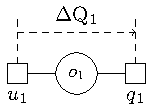
\includegraphics[scale=1.2]{tikz/outdq.pdf}
        \end{center}
        \caption{The outcome (circle) and the starting set (left) and terminating set (right) of events. \cite{myo}}
    \end{figure}

\subsection{Quality attenuation ($\Delta$Q)}
        Assume a component $C$ which receives a message $m_{in}$ and outputs a message $m_{out}$ after a delay $d$. Over multiple executions, we will have observed multiple delays which can be represented as a cumulative definition where $p$ percent of delays have delay $\le d$. \cite{art} 

        \textbf{$\Delta$Q} is a cumulative distribution function that defines both \textit{latency} and \textit{failure probability} between a start and end event. \cite{dq-tut}

        In an ideal system, an outcome would deliver a desired behaviour without error, failure, delay, but this is not the case. The quality of an outcome response "attenuated to the relative ideal" (the cumulative distribution function) is called "quality attenuation" ($\Delta$Q) and can depend on many factors (geographical, physical \dots). Its distribution may be modelled by a random variable.

    As $\Delta$Q captures deviation from ideal behavior and incorporates delay, which is a continuous random variable, and failures/timeouts, which are discrete variables, it can be described mathematically as an \textit{Improper Random Variable}, where the probability of a finite or bounded delay $<$ 1. 

    \textbf{$\Delta$Q(x)} is the probability that an outcome $O$ occurs in time $t \le x$. The \textbf{\textit{intangible mass}} $1 - \lim_{x\to\infty}\Delta Q(x)$ of a $\Delta$Q will encode the probability of failure/timeout/exception occuring. \cite{myo}
    
    \begin{figure}[H]
        \begin{center}
            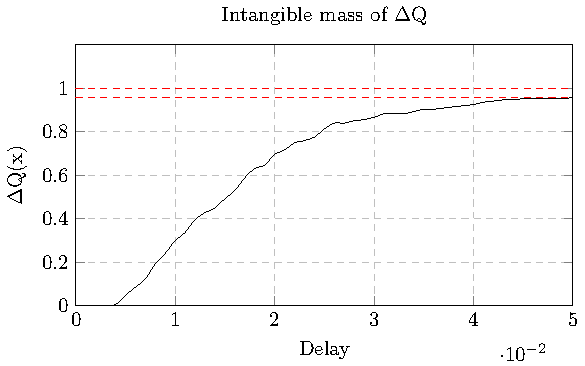
\includegraphics{tikz/intangible.pdf}
        \end{center}
        \caption{Intangible mass (red) of a $\Delta$Q with failure rate of about 5\% }
    \end{figure}
   
  \subsection{Failure semantics}
       In the CDF representation of a $\Delta$Q, there is an \textit{f} percent probability that the delay is infinite, this is what failure models. 
        Concretely, it means that an input message $m_{in}$ \textbf{has no output message} $m_{out}$. \cite{art}

        Combining delay and failure in a single quantity is what makes $\Delta$QSD a great choice to explore feasibility in system design. \cite{dq-tut}
   
    \subsection{Partial ordering}
        A CDF of a $\Delta$Q is \textit{less than} the other if its CDF is everywhere to the left and above the other. Mathematically, it is a partial order. 
        
        If two $\Delta$Qs intersect, they are not ordered. \cite{dq-tut}

    \subsection{Timeliness}
        Timeliness is defined as a relation between an observed $\Delta Q_{obs}$ and a required $\Delta Q_{req}$. Timeliness is delivering results within required time bounds (sufficiently often). 

        A system \textit{satisfies timeliness} if $\Delta$Q$_{obs}$ $\le$ $\Delta$Q$_{req}$. \cite{art}
     
    \subsection{QTA, required $\Delta$Q}
         The \textit{Quantitative Timeliness Agreement} (QTA) maps objective measurements to the subjective perception of application performance. It specifies what the base system does and its limits. \cite{dq-br}
    
    \paragraph{Slack} There is performance \textit{slack} when a $\Delta$Q is strictly less than the requirement,

        \paragraph{Hazard} There is performance \textit{hazard} when a $\Delta$Q is strictly greater than the requirement. \cite{myo}
    
    \paragraph{QTA example}: Imagine a system where 25\% of the executions should take $<$ 15 ms, 50\% $<$ 25 ms and 75\% $<$ 35 ms, all queries have a maximum delay of 50ms and 5\% of executions can timeout, the QTA can be represented as a step function.
    
        \begin{figure}[H]
            \begin{center}
                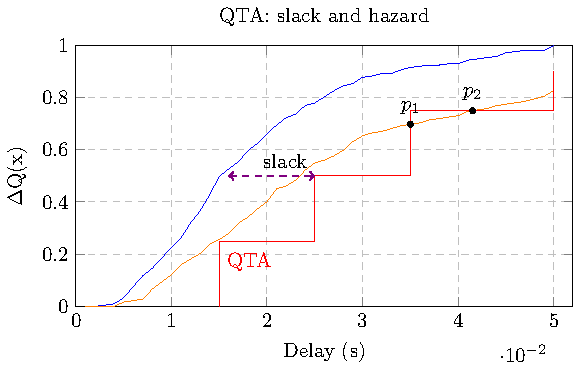
\includegraphics[scale=1]{tikz/cdf_qta_slack.pdf}
            \end{center}
            \caption{The system in blue is showing slack and satisfies the requirement. The system in orange is showing signs that it cannot handle the stress, it is not respecting the system requirements imposed by the QTA.}%
        \end{figure}

    \subsection{Outcome diagram}
        An outcome diagram is central to capture the causal relationships between the outcomes. It shows the causal connections between all the outcomes we are interested in, and it allows computing the $\Delta$Q for the whole system \cite{dq-tut}. It maps a system's behaviour as seen from outside to concrete outcomes \cite{art}.
        There are four different operators that represent the relationships between outcomes. \cite{dq-tut}

    \subsubsection{Sequential composition}
        If we assume two outcomes $O_A$, $O_B$ where the end event of $O_A$ is the start event of $O_B$, the two outcomes can be sequentially composed. The total delay $\Delta$Q$_{AB}$ is given by the convolution of the PDFs of $O_A$ and $O_B$ ($O_A \circledast O_B$).
        
        \begin{figure}[H]
            \begin{center}
                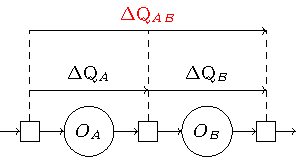
\includegraphics[scale=1]{tikz/seq_comp.pdf}
            \end{center}
            \caption{Sequential composition of $O_A$ and $O_B$.}
        \end{figure}
        Where convolution ($\circledast$) between two PDF is:
        \begin{equation}
            PDF_{AB}(t) =\int\limits_0^t PDF_A(\delta) \cdot PDF_B(t-\delta)d\delta 
            \label{eq:conv_1}
        \end{equation}

        Thus, $\Delta$Q$_{AB}$:
        \begin{equation}
            \Delta Q_{AB} = PDF_{A} \circledast PDF_{B}
            \label{eq:convolution_pdf}
        \end{equation}

        Convolution is the only operation which is based on the PDFs, the following operations are based on the CDF of the $\Delta$Qs (hence the use of the $\Delta$Q notation).
        
    \subsubsection{First to finish (FTF)}
            If we assume two independent outcomes $O_A$, $O_B$ with the same start event, first-to-finish occurs when at least one end event occurs, it can be calculated as:
        \begin{equation}
            \begin{split}
                \Delta Q_{FTF(A, B)} &= Pr[d_A > t \wedge d_B > t] \\
                & = Pr[d_A > t] \cdot Pr[d_B > t] = (1 - \Delta Q_A) \cdot (1 - \Delta Q_B) \\
                \Delta Q_{FTF(A, B)} &= \Delta Q_A + \Delta Q_B - \Delta Q_A \cdot \Delta Q_B  
            \end{split}    
            \label{eq:ftf} 
        \end{equation}

       \begin{figure}[H]
            \centering
            \begin{subfigure}{.5\textwidth}
                \centering
                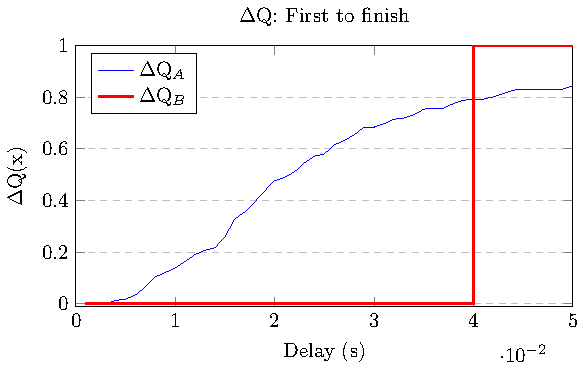
\includegraphics[scale = 0.7]{tikz/ftf_1.pdf}
                \label{fig:ftf1}
            \end{subfigure}%
            \begin{subfigure}{.5\textwidth}
                \centering
                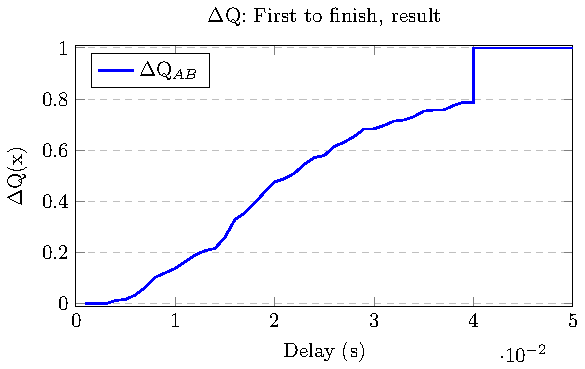
\includegraphics[scale = 0.7]{tikz/ftf_2.pdf}
                \label{fig:ftf2}
            \end{subfigure}
            \caption{Left: $\Delta$Q$_{(A, B)}$. Right: FTF$_{(A, B)}$ = $\Delta$Q$_{AB}$}%
            \label{fig:ftf}
            \end{figure}


    \subsubsection{All to finish (ATF)}
        If we assume two independent outcomes $O_A$, $O_B$ with the same start event, all-to-finish occurs when both end events occur, it can be calculated as:
        \begin{equation}
            \begin{split}
                \Delta Q_{ATF(A, B)} &= Pr[d_A \le t \wedge d_B \le t] \\
                & = Pr[d_A \le t] \cdot Pr[d_B \le t] = \Delta Q_A \cdot \Delta Q_B \\
                \Delta Q_{ATF(A, B)} &= \Delta Q_A \cdot \Delta Q_B 
            \end{split}
            \label{eq:atf}
        \end{equation}
        
        \begin{figure}[H]
            \centering
            \begin{subfigure}{.5\textwidth}
                \centering
                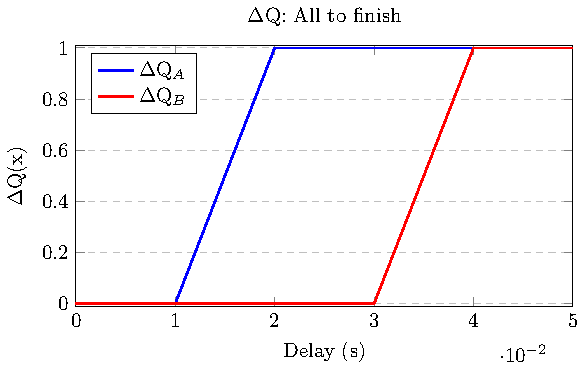
\includegraphics[scale = 0.7]{tikz/atf_1.pdf}
                \label{fig:atf_1}
            \end{subfigure}%
            \begin{subfigure}{.5\textwidth}
                \centering
                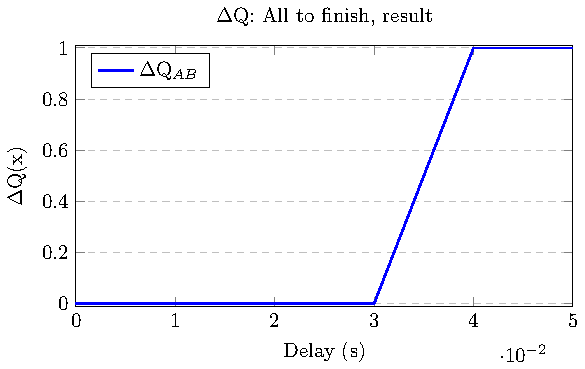
\includegraphics[scale = 0.7]{tikz/atf_2.pdf}
                \label{fig:atf2}
            \end{subfigure}
            \caption{Left: $\Delta$Q$_{(A, B)}$. Right: ATF$_{(A, B)}$ = $\Delta$Q$_{AB}$}%
            \label{fig:atf}
            \end{figure}

    \subsubsection{Probabilistic choice (PC)}
        If we assume two possible outcomes $O_A$ and $O_B$ and exactly one outcome is chosen during each occurence of a start event and:
        \begin{itemize}
            \item $O_A$ happens with probability $\dfrac{p}{p+q}$
            \item $O_B$ happens with probability $\dfrac{q}{p + q}$
        \end{itemize}
        \begin{equation}
           \Delta Q_{PC}(A, B) = \dfrac{p}{p + q}\Delta Q_A + \dfrac{q}{p + q}\Delta Q_B 
            \label{eq:pc}
        \end{equation} 

    \begin{figure}[H]
        \begin{center}
            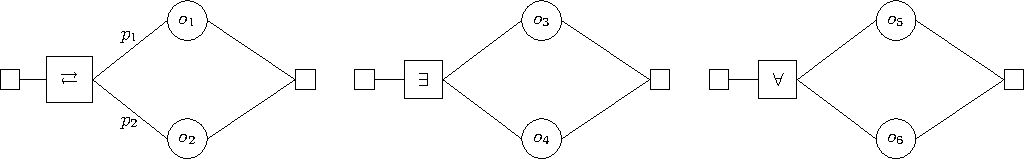
\includegraphics[width = \textwidth]{tikz/op.pdf}
        \end{center}
        \caption{The possible operators in an outcome diagram: Probabilistic choice, first-to-finish, all-to-finish}
        \label{fig:op}
    \end{figure}
    First-to-finish, All-to-finish and probabilistic-choice are calculated on the CDF of the $\Delta$Q of their components.
    
    These operators can be assembled together to create an outcome diagram, later on, we will see how one can go from the graphical representation to outcome diagrams which can be used in the $\Delta$Q oscilloscope.
    
    \subsection{Outcome diagrams refinement}
        An important feature of outcome diagrams is the ability to be able to design a system even with \textit{"black-boxes"}, before the complete details of it are known. \\
        An outcome diagram can be "unboxed" by refining the outcomes that compose it. We can adapt a situation described in Mind your Outcomes to understand how refinement can allow the user to have a very precise representation of a system. \cite{myo}
        
        We first start with a black-box, unnamed outcome with start event $A$ and end event $Z$, somewhere in the system. The first refinement step would be giving the outcome a name.

      \begin{figure}[H]
            \begin{center}
                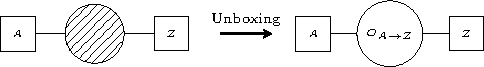
\includegraphics[scale = 1]{tikz/black_box.pdf}
            \end{center}
            \caption{Refinement from black box to named outcome.}
            \label{fig:bb}
        \end{figure}

    The system can be further refined by adding outcomes that represent tasks. For example, the engineer might believe that it will take two tasks to get from A to Z. We can then add another outcome, sequentially composed, to represent this situation.

       \begin{figure}[H]
            \begin{center}
                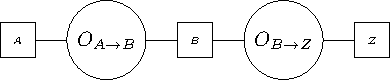
\includegraphics[scale = 1]{tikz/out_2.pdf}
            \end{center}
            \caption{Further refinement from one task to two tasks.}
            \label{fig:2_hops}
        \end{figure}

        We can also model the chance of executing two tasks as a probabilistic choice, where there is $p_2$ probability that the execution from A to Z will execute two tasks. The outcome diagram can be refined as a probabilistic choice.

   \begin{figure}[H]
            \begin{center}
                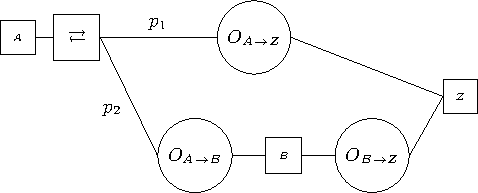
\includegraphics[scale = 1]{tikz/ref_op.pdf}
            \end{center}
            \caption{Refinement as probabilistic choice of executing either one or two tasks.}
            \label{fig:prob_ref}
        \end{figure}
    In essence, the refinement could model a very fine-grained representation of the system by further refining the system, to represent the possibility of executing $n$ tasks. This demonstrates the power of outcome diagrams to represent system diagrams with high precision. They can help explore design decisions thanks to outcomes and operators.

    \subsection{Independence hypothesis}  
        An important aspect of sequential composition is the assumption of outcomes having independent behaviour. Let us explain the following assumption clearly.

        Assume two sequentially composed outcomes $o_1$, $o_2$ running on the same processor. The overall delay of execution can be observed from the start event of $o_1$ ($u_1$) to the end event of $o_2$ ($r_1$). 
        \begin{figure}[H]
            \begin{center}
                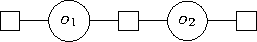
\includegraphics[scale=1]{tikz/indep.pdf}
            \end{center}
        \end{figure}
        
        At low load, the two components behavior will be independent, the system will behave \textbf{linearly}. According to the superposition principle, the overall delay will be the sum of the two delays, as will the overall processor utilisation. \cite{sup-p}
        
        When load increases, the two components will start to show dependent behaviour due to the processor utilisation increasing. The $\Delta$Q of the observed total delay will then deviate from the sum of the two delays ($o_1 \circledast o_2$). 
        
        \begin{figure}[H]
            \begin{center}
                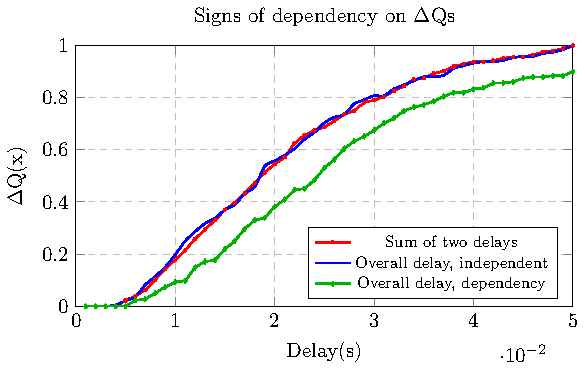
\includegraphics[scale=1]{tikz/cdf_indep.pdf}
            \end{center}
            \caption{When the components are independent, the sum of the two delays (blue) and the overall delay (red) can be superposed. \\
            When $o_1$ and $o_2$ show initial signs of dependency, the overall delay (green) can be seen deviating from the sum of the two delays.}
            \label{fig:cdf_indep}
        \end{figure}

        When the system is far from being overloaded, the effect is noticeable thanks to $\Delta$QSD. As the cliff edge of overload is approached, the nonlinearity will increase \cite{post}. These theoretical results can be observed in practice in the oscilloscope. We will explore such cases in the synthetic applications section.

    \section{Observability}
    OpenTelemetry refers to observability as \cite{otel-o}:
    \begin{quote}
 ``The ability to understand the internal state by examining its output. In the context of a distributed system, being able to understand the internal state of the system by examining its telemetry data.''
    \end{quote}
    In the case of the Erlang programming language, we describe respectively two different ways to observe a running Erlang system: erlang:trace and OpenTelemetry.
    
    \subsection{erlang:trace}
        The Erlang programming language gives the users different ways to observe the behaviour of a system, one of those is the interface \texttt{erlang:trace}. According to the documentation: ``The Erlang run-time system exposes several trace points that can be observed, observing the trace points allows users to be notified when they are triggered'' \cite{erl-t}. One can observe function calls, messages being sent and received, process being spawned, garbage collecting \dots. 
        \begin{figure}[!ht]
        \centering
        \begin{minted}{erlang}
            -spec trace(PidPortSpec, How, FlagList) -> integer()
               when
                   PidPortSpec ::
                       pid() |
                       port() |
                       all | processes | ports | existing | existing_processes | existing_ports | new |
                       new_processes | new_ports,
                   How :: boolean(),
                   FlagList :: [trace_flag()].
        \end{minted}
        \caption{erlang:trace/3 specification.}
\end{figure}

    Nevertheless, in Erlang trace there is no default way to follow a message and get its whole execution trace. This is a missing feature that is crucial for observing a program functioning and being able to connect an application to our oscilloscope.  This is where the OpenTelemetry framework comes in.

\subsection{OpenTelemetry}
    According to OpenTelemetry website \cite{otel-o}: OpenTelemetry is an open-source, vendor-agnostic observability framework and toolkit designed to generate, export and collect telemetry data, in particular traces, metrics and logs. OpenTelemetry provides a standard protocol, a single set of API and conventions and lets the user own the generated data, allowing to switch between observability backends freely.
   
   OpenTelemetry is available for a plethora of languages \cite{otel-l}, including Erlang, although, as of writing this, only traces are available in Erlang \cite{otel-in}.
     
    The Erlang Ecosystem Foundation has a working group focused on evolving the tools related to observability, including OpenTelemetry and the runtime observability monitoring tools \cite{obs-group}. 
    
    \subsubsection{Traces}
        Traces are why we are basing our program on top of OpenTelemetry, traces follow the whole path of a request in an application, and they are comprised of one or more spans. Traces can propagate to multiple services and record multiple paths in different microservices \cite{otel-dt}. 
        
        \paragraph{Span} A span is a unit of work or operation. Multiple spans can be assembled into a trace and can be causally linked (\cref{fig:monitor}). The spans can have a hierarchy, where \textit{root spans} represent a request from start to finish and a child span the requests that are completed inside the root span \cite{otel-dt}. We will see in later sections how this can relate to what the oscilloscope does.

    The notion of spans and traces allows us to follow the execution of a request and carry a context. Spans can be linked to mark causal relationships between multiple spans \cite{otel-t}. This relation can be represented in the oscilloscope via \textbf{probes}, we will present how spans relate to probes in following sections.
    \begin{figure}[H]
    \begin{minted}{json} 
{
  "name": "oscilloscope-span",
  "context": {
    "trace_id": "5b8aa5a2d2c872e8321cf37308d69df2",
    "span_id": "5fb397be34d26b51"
  },
  "parent_id": "051581bf3cb55c13",
  "start_time": "2022-04-29T18:52:58.114304Z",
  "end_time": "2022-04-29T22:52:58.114561Z",
  "attributes": {
    "http.route": "some_route"
  },
}
    \end{minted}
    \caption{Example of span from the OpenTelemetry website \cite{otel-t}. The span has a parent, indicating that child and parent spans are related and are both part of the same trace.}%
    \end{figure}

    \subsubsection{Monitoring OpenTelemetry spans}
        In OpenTelemetry, the user can export their traces export to backends and monitoring such as Jaeger (\cref{fig:monitor}), Zipkin, Datadog \cite{otel-exp}. There, a user can analyse the traces to troubleshoot their programs by observing the flow of the requests \cite{jg}. These monitoring tools give extensive details about a running system, but may fail to capture essential timeliness requirements and performances issues early enough.
        
        Our oscilloscope is a kind of monitoring tool, one that gives precise statistical insights about a running system. It is clear that the oscilloscope does not have the same capabilities as Datadog \cite{datadog} might have, where you can observe cloud instances, instances cost, dependency graphs \dots but the oscilloscope can nevertheless provide precise insights about dependency, overload thanks to the $\Delta$QSD paradigm. 

        This is also the reason why the adapter includes OpenTelemetry macros. The oscilloscope can be put next to a monitoring tool where one might export spans to, so that an engineer might consult the monitoring tool to get the global picture of a running app. The oscilloscope provides more precise insights to understand the system's behaviour. 
       \begin{figure}[H]
            \centering
            \begin{subfigure}{.5\textwidth}
                \centering
                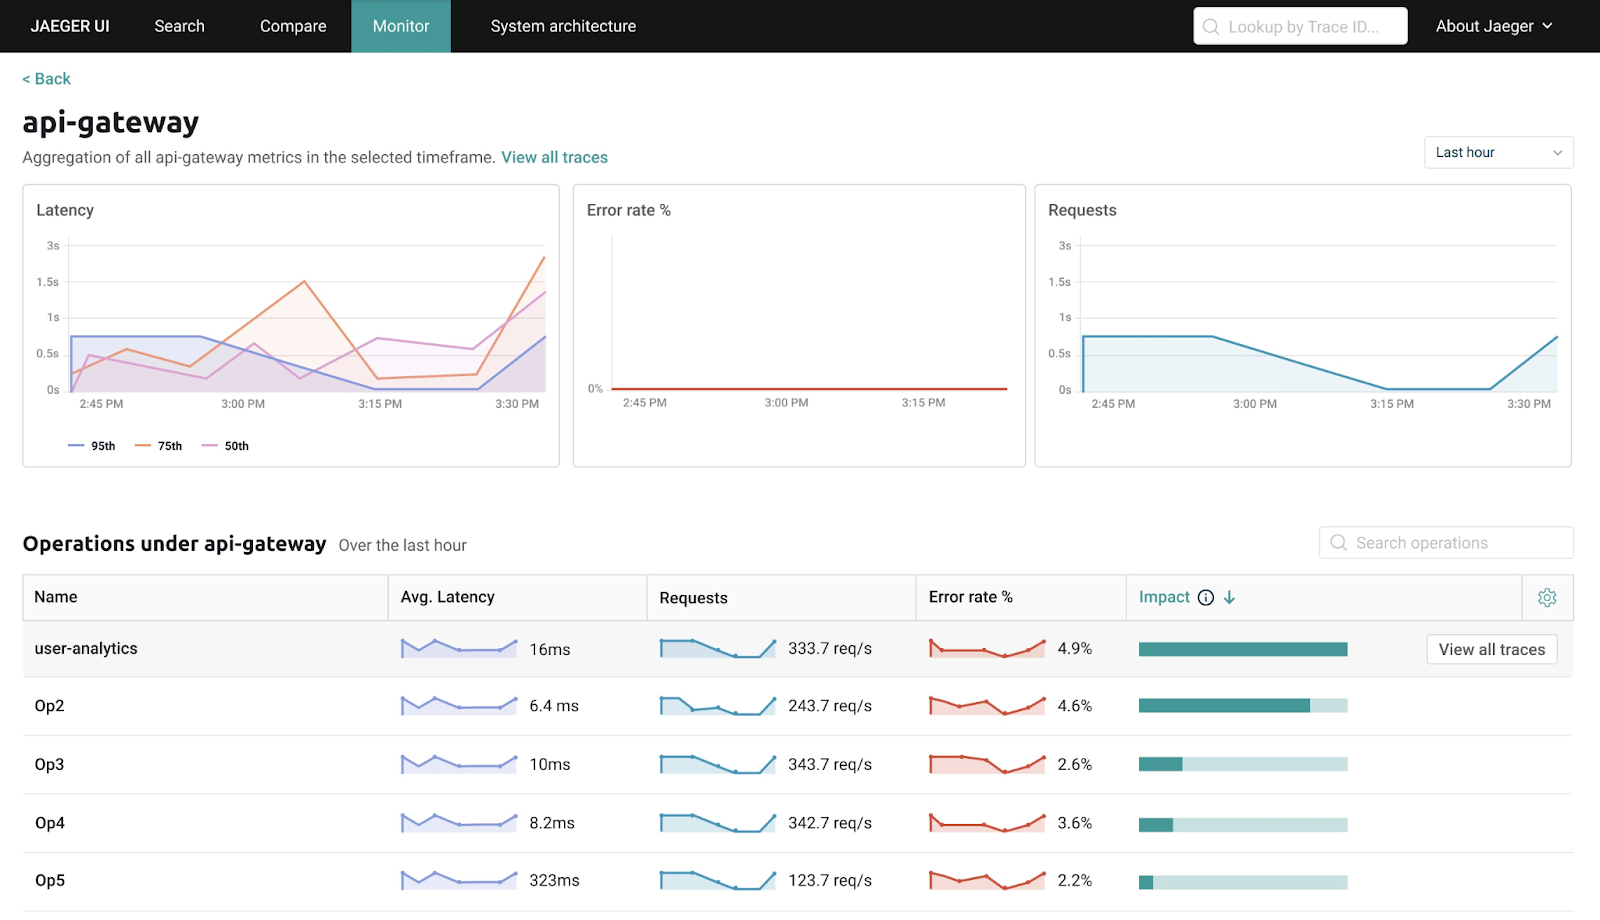
\includegraphics[width=0.98\textwidth]{img/jaeger.png}
                \label{fig:jag}
            \end{subfigure}%
            \begin{subfigure}{.5\textwidth}
                \centering
                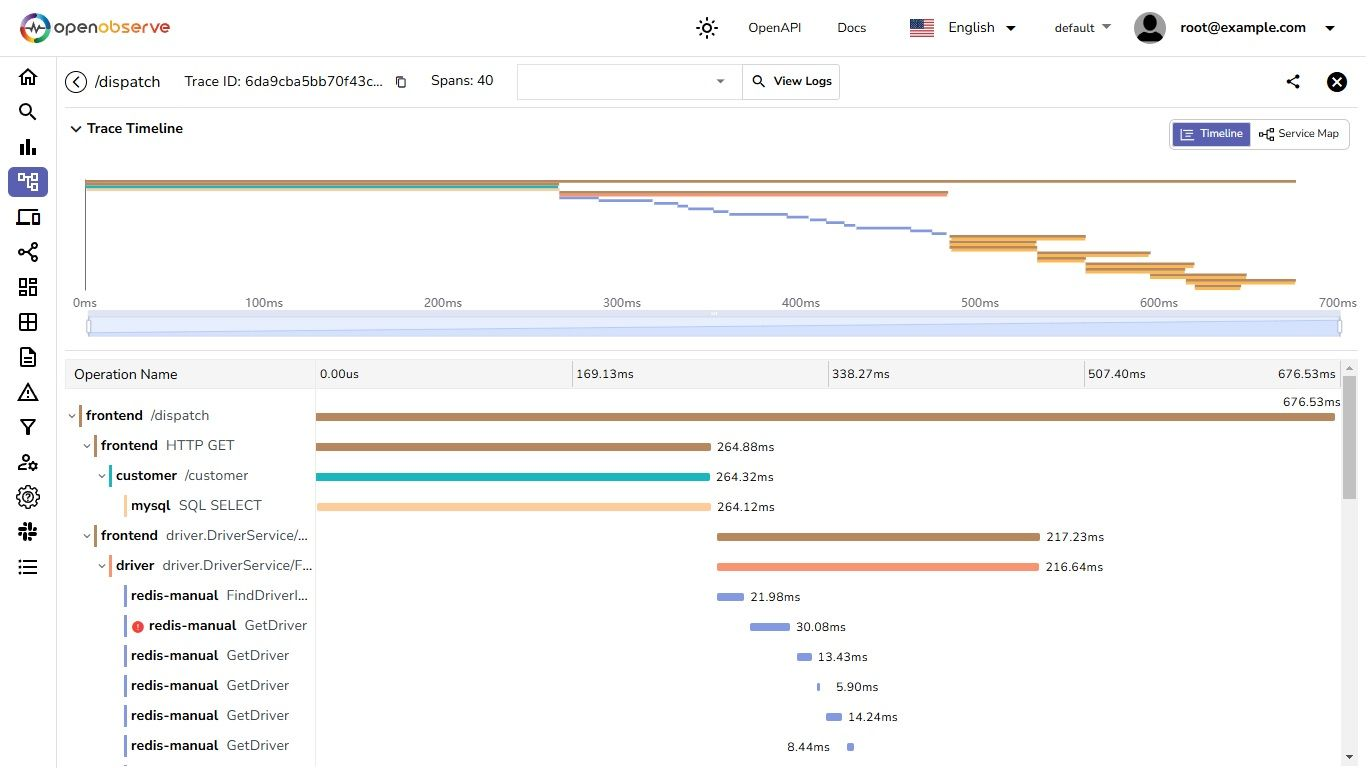
\includegraphics[width =0.98\textwidth]{img/jaeger2.jpg}
                \label{fig:openobs}
            \end{subfigure}
            \caption{Left: Jaeger interface. Right: Analysis of a span on OpenObserve.}
            \label{fig:monitor}
            \end{figure}

    \subsubsection{Span macros}
        OpenTelemetry provides macros to start, end and interact with spans in Erlang, the following code excerpts are taken from the OpenTelemetry instrumentation wiki. \cite{otel-in}
        \paragraph{?with\_span}
            \texttt{?with\_span} creates active spans. An active span is the span that is currently set in the execution context and is considered the ``current'' span for the ongoing operation or thread. \cite{active-s}
        \begin{minted}{erlang}
parent_function() ->
    ?with_span(parent, #{}, fun child_function/0).
child_function() ->
    %% this is the same process, so the span parent set as the active
    %% span in the with_span call above will be the active span in this function
    ?with_span(child, #{},
               fun() ->
                   %% do work here. when this function returns, child will complete.
               end).
        \end{minted}
        \paragraph{?start\_span}
            \texttt{?start\_span} creates a span which isn't connected to a particular process, it does not set the span as the current active span.
        \begin{minted}{erlang}
SpanCtx = ?start_span(child),
Ctx = otel_ctx:get_current(),
proc_lib:spawn_link(fun() ->
                        otel_ctx:attach(Ctx),
                        ?set_current_span(SpanCtx),
                        ?end_span(SpanCtx)
                    end),
        \end{minted}
        \paragraph{?end\_span}
            \texttt{?end\_span} ends a span started with \texttt{?start\_span}


    \section{Current observability problems}

    A legitimate question to pose would be why one would need an additional tool to observe their system, monitoring tools are already plenty and provide useful insights into an application's behaviour. While they may seem adequate to provide a global oversight of applications, they fail to diagnose real time problems like overload, dependent behaviour early enough and in a quick manner.

    The problem we are trying to tackle can be described by the following situation: 
    Imagine an Erlang application instrumented with OpenTelemetry, suddenly, the application starts slowing down, and the execution of a function takes 10 seconds instead of the usual 1 second. Between its start and its end, the user instrumenting the application sees nothing in their dashboard.
    
    This is a big problem! One would like to know right away if something is wrong with their application, better! Even before problems are apparent. This is where the $\Delta$QSD paradigm and the $\Delta$Q oscilloscope come in handy.
   
   By leveraging $\Delta$QSD notion of failure and QTAs, problems can be detected right away in the oscilloscope. 
    
    \begin{figure}[H]
        \begin{center}
            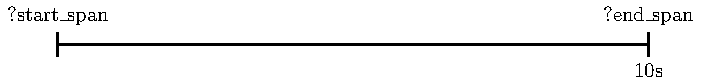
\includegraphics{tikz/start_end.pdf}
        \end{center}
        \caption{Execution of a long span in OpenTelemetry, the user will only be notified after 10 seconds that the function has ended (and taken too long).}
    \end{figure}

    \begin{figure}[H]
        \begin{center}
            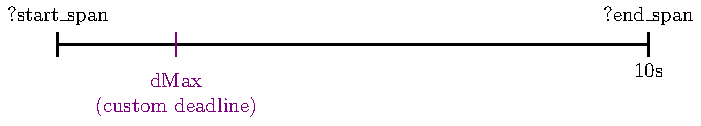
\includegraphics{tikz/start_end_dmax.pdf}
        \end{center}
        \caption{Execution of a long span in OpenTelemetry, the $dMax$ deadline allows knowing that the span has taken too long.}
        \label{fig:otel_dmax}
    \end{figure} 


    \subsection{Handling of long spans}
        OpenTelemetry presents a bigger problem, what happens when there are long-running spans? Worse, what happens when spans are not actually terminated?
        
        OpenTelemetry limits the length of its spans, moreover, those who are not terminated are lost and not exported. Why? Failed executions are those that tell more about a program's execution!

        If the span is the parent/root span, its effect could trickle down to child spans. We can quickly see how this becomes problematic, all the information about an execution of your program \dots lost. Moreover, a span could not be terminated for trivial reasons: refreshing a tab, network failures, crashes \dots \cite{otel-l}. There are a few hacks that can be implemented, having shorter spans, carrying data in child spans, saving spans in a log to track spans which were not ended to manually set an end time; why the need to circumvent limitations when observing a system?

     We believe that the adapter we provide can be a great start to improve observability requirements surrounding OpenTelemetry. We will show in the evaluation on synthetic applications how $\Delta$QSD's notion of failure can help to detect overload problems in running systems right away.


    \chapter{Design}
    This chapter aims to first extend the concepts of $\Delta$QSD, giving more insights into how the systems need to be instrumented to correctly work together, and how the different parts need to be integrated to interact together.
    \begin{itemize}
        \item We first provide concepts of probes, we extend the $\Delta$QSD notion of failure and describe how time series will work in our oscilloscope, this part is crucial to understand how the measurements are done in real time.
        \item We then explain the global design of the system (see \cref{fig:sys_diag}) in two parts: \\
            Firstly, we explain the application side, where the Erlang running system is. Consequently, it's where the $\Delta$Q adapter interface will be. It performs the translation of spans to outcome instances thanks to the inserted probes. \\
            Secondly, the oscilloscope side. There, the server receives information about outcome instances from the adapter. The $\Delta$Q oscilloscope can then plot $\Delta$Q graphs from the instances. In the oscilloscope one can define outcome diagrams, set parameters for probes and control the adapter.
        \item Lastly, we provide high level concepts of execution windows, triggers and snapshot. These are the key design elements of the oscilloscope. 
    \end{itemize}

    \begin{figure}[H]
        \begin{center}
            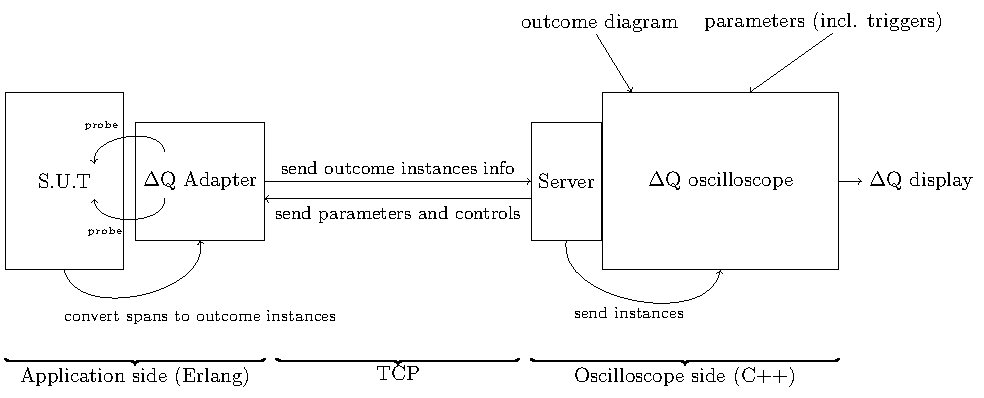
\includegraphics[scale = 0.8]{tikz/sut-stub-osc.pdf}
        \end{center}
        \caption{Global system design diagram. The two sides communicate via TCP sockets to share information about outcome instances and probe parameters.}
        \label{fig:sys_diag}
    \end{figure}

    \section{Measurement concepts}
    \subsection{Probes}

A system instrumented with OpenTelemetry has spans and traces to observe the execution of an operation \cite{otel-t}. The same level of observability must be assured in the oscilloscope, this is why we provide the concept of probes, which, like spans, follow an execution from start to end. \textbf{Note} that a definition of probes has already been introduced in a previous article relating to $\Delta$QSD \cite{dq-br}, but the concept we present here is not the same.

To observe a system, we must put probes in it. For each outcome of interest, a probe (observation point) is attached to measure the delay of the outcome, like one would in a true oscilloscope \cite{post}.

Consider \cref{fig:probes} below. A probe is attached at every component (for example, a database \cite{dq-tut}) to measure their $\Delta$Qs ($p_2, p_3$). Another probe ($p_1$) is inserted at the beginning and end of the system to measure the global execution delay. Thanks to this probe, the user can observe the $\Delta$Q \textit{``observed at $p_1$''}, which is the $\Delta$Q which was calculated from the data received by inserting probe $p_1$. The \textit{$\Delta$Q ``calculated at $p_1$''} is the resulting $\Delta$Q from the convolution of the observed $\Delta$Qs at $c_2$ and $c_3$. \\
Probe $p_1$ is the equivalent of a ``root/parent span'' which observe the whole execution of $c_1, c_2$, while $p_2$ and $p_3$ are child spans which represent single instances of execution.

    \begin{figure}[H]
        \begin{center}
            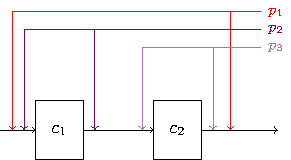
\includegraphics[scale=1.8]{tikz/probes.pdf}
        \end{center}
        \caption{Probes inserted in a component diagram. In an application instrumented with OpenTelemetry, $p_1$ could be considered the root span, $c_1$ and $c_2$ its children spans sharing a causal link.}
        \label{fig:probes}
    \end{figure}




    \subsection{Extending failure}
   Recall the definition of failure: \textit{``an input message $m_{in}$ that has no output message $m_{out}$''} \cite{art}. In the previous section \ref{fig:otel_dmax}, we also introduced the notion of a maximum delay. 

   By extending the notion of failure to include $dMax$, we can know right away when execution is straying away from engineer defined behaviour, avoiding having to wait until the execution is done. In $\Delta$QSD, an execution may as well take 10 or 15 seconds, but if the delay of execution is $> dMax$, we consider that \textbf{failed} right away, we do not need to know the total execution time, the execution has already taken too much \cite{myo}. The full span will be exported regardless to monitoring tools which were set up by the user. 

   The user can observe both real time information with $\Delta$QSD notion of failure on the $\Delta$Q oscilloscope, and observe those spans in their monitoring tools if they wish.

The notion of failure is extended to the following definition:
        \begin{center}
            \textit{``An input message $m_{in}$ that has no output message $m_{out}$ after $dMax$''} 
        \end{center}
    We can leverage this new definition to observe the system and the $\Delta$Qs in real time.


    \subsection{Time series of outcome instances}
    Consider a probe $p$ with two distinct sets of events, the starting set of events $s$ and ending set of event $e$. The outcome instance of a message $m_s \rightarrow m_e$ contains:
    \begin{itemize}
        \item The probe's $p$ name
        \item The start time $t_s$
        \item The end time $t_e$
        \item Its status 
        \item Its elapsed time of execution
    \end{itemize}
    The instance has three possible statuses: \texttt{success, timeout, failure}, it can thus be broken down in the representations, based on its status:
    \begin{itemize}
        \item \textbf{($t_s$,$t_e$)}: This representation indicates that the execution was successful (t $<$ $dMax$). 
        \item \textbf{($t_s, \mathcal{T}$)}: This representation indicates that the execution has timed out (t $>$ $dMax$). The end time and elapsed time is equal to $t_s + \text{timeout}$ 
        \item \textbf{($t_s, \mathcal{F}$)}: This representation indicates the execution has failed given a user defined requirement (i.e. a dropped message given buffer overload in a queue system). It must not be confused with a program failure (crash), if a program crashes during the execution of event $e$, it will time out since the adapter will not receive an end message.
    \end{itemize}
    The \textbf{time series} of a probe is the sequence of $n$ outcome instances and can then be easily modeled by $\Delta$Q.

    \paragraph{What can be considered a failed execution?} Imagine a queue with a buffer: the buffer queue being full and dropping incoming messages can be modeled as a failure.

    More generally, the choice of what is considered a failed execution is left up to the user who is handling the spans and is program-dependent. Exceptions or errors can be kinds of failure. 

    On another note, the way of handling errored spans in OpenTelemetry can differ from user to user, so the adapter will not handle ending and setting statuses for "failed" spans. \cite{otel-err}
   
   In any case, by the new definition of failure, \textbf{timed out and failed will both be considered as a failure} in the calculation of a $\Delta$Q.

    \section{Application side} 
    \subsection{System under test} The system under test \textbf{(S.U.T)} is the Erlang system the engineer wishes to observe (\cref{fig:sys_diag}). It ideally is a system which already is instrumented with OpenTelemetry. The ideal system where $\Delta$QSD is more useful is a system that executes many independent instances of the same action \cite{dq-tut}. 
    
    \subsection{$\Delta$Q Adapter} 
    The $\Delta$Q adapter is the \texttt{dqsd\_otel} Erlang interface \cite{wrapper}. It starts and ends OpenTelemetry spans and translates them to outcome instances which are useful for the oscilloscope. This can be done thanks to probes being attached to the system under test, like an oscilloscope would. The outcome instances end normally like OpenTelemetry spans or, additionally, can timeout after a custom timeout ($dMax$), and fail, \textit{according to user's definition of failure}. 
    
    Handling of OpenTelemetry spans which goes beyond starting and ending them is delegated to the user, who may wish to do further operations with their spans. 
    The adapter is called from the system under test and communicates outcome instances data to the oscilloscope via TCP sockets. 
    
    The adapter can receive messages from the oscilloscope, the messages are about updating probe's $dMax$ or starting and stopping the sending of data to the oscilloscope.
    \subsection{Inserting probes in Erlang - From spans to outcome instances}
        OpenTelemetry spans are useful to carry context, attributes and baggage in a program \cite{otel-dt}. The plethora of attributes they have is nevertheless too much for the oscilloscope. 
        To get the equivalent of spans for the oscilloscope, the adapter needs to be called at the starting events of a probe to start an instance of a probe, and at the ending events to end the outcome instance. The name given with \texttt{``start\_span/with\_span''} is the name of the probe. The PID which is returned by starting a span must be carried throughout the whole execution, and used when ending spans to create the correlation between a probe and an outcome instance.
\begin{figure}[H]
\centering
   \begin{minted}{erlang}
        % Start the outcome instance of probe. The call to dqsd_otel starts an OpenTelemetry span, as it contains a call to ?start_span(Name)
        {ProbeCtx, ProbePid} = dqsd_otel:start_span(<<"probe">>),  

        % Start and fail span directly
        {WorkerCtx, WorkerPid} = dqsd_otel:start_span(<<"worker_1">>),   
        dqsd_otel:fail_span(WorkerPid),
        %Here, you would need to end the span manually with ?end_span

        %Example of with_span, the call to OpenTelemetry ?with_span is inside the adapter function, the function fun() -> ok end is executed inside dqsd_otel.
        dqsd_otel:with_span(<<"worker_2">>, fun() -> ok end), 
        %End the outcome instance of probe. This ends the OpenTelemetry span aswell. If the outcome instance has already timed out (the time from start_span to end_span > dMax), the oscilloscope receives no message where the status is successful. Otherwise, this sends a message with startTime, endTime, the name "probe" and success status.
        dqsd_otel:end_span(ProbeCtx, ProbePid),
        \end{minted}
\caption{Example usage of the adapter}\label{code:adapter}
\end{figure}
    Further details about the implementation of the adapter are explained in Chapter 5. A user guide on how to include the adapter in your project and how to instrument a program is found in the appendix (\cref{app:instr_app}). 
  
    \section{Oscilloscope side}
    \subsection{Server} The server is responsible for receiving the messages containing the outcome instances from the adapter. The server forwards the instances to the oscilloscope.
    
    \subsection{$\Delta$Q Oscilloscope} The oscilloscope is a C++ graphical application which implements a dashboard to observe $\Delta$Qs of probes inserted in the system under test \cite{osc-g}. It receives the instances corresponding to probes from the server and adds them to the time series of the probes whose instance is being received. 
    The oscilloscope has a graphical interface which allows the user to create an outcome diagram of the system under test, display real time graphs which show detail about the execution of the system and allow the user to set parameters for probes. It can also display snapshots of the system as if it was frozen in time.

    \subsection{Inserting probes in the oscilloscope}
        Probes are automatically inserted in the oscilloscope when creating outcome diagrams. They are inserted on the outcomes observables, operators observables and to the sub-outcome diagrams observables (probes that observe the causal links of multiple outcomes/operators), we will see later on how they can be defined and how an outcome diagram can be created. \\
    The names that are given to outcome, operators and sub-outcome diagrams are the names of the probes that observe them. Giving these probes a name allows the oscilloscope to match the outcome instances to the probes' time series.

        In the system below, which is equal to the one defined above, probes are automatically attached to outcomes $o_1, o_2$. The user who wants to observe the result of the sequential composition can insert probes at the start and end of the routine. 
    
        \begin{figure}[H]
            \begin{center}
                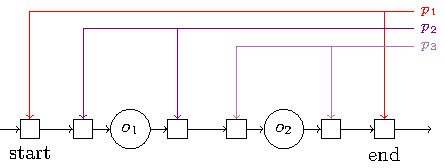
\includegraphics[scale=1.3]{tikz/probe_1.pdf}
            \end{center}
            \label{fig:probes_o}
            \caption{Probes inserted in the outcome diagram of the previous component diagram in \cref{fig:probes}.}
        \end{figure}
       
    The \textbf{observables} are an abstract representation of events. Consider the previous code snippet \cref{code:adapter}: the $start$ event of ``probe'' and worker$_1$'s start event are subsequent instructions. The probe's start event is practically the same as worker$_1$'s start event, indeed, they could be overlapped in the graph above. We nevertheless show the distinction to show that probe and worker$_1$ need to be started differently in Erlang as the information they carry is about two distinct instances. Furthermore, this difference is remarked in the definition of outcome diagrams, for which we provide a syntax in the following chapter. 
    
    As for operators, probes are automatically attached to the components inside them and to the start event and end events of the operators (its observables). 

       \begin{figure}[H]
           \begin{center}
                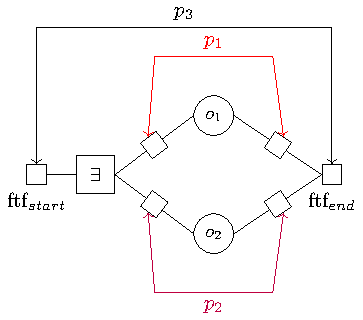
\includegraphics[scale = 1.3]{tikz/probe_2.pdf}
            \end{center}
            \label{fig:probes_op}
            \caption{Probes inserted into an operator.}
       \end{figure}
    
    The \textbf{observed $\Delta$Q} for the first-to-finish operator is the $\Delta$Q for the observables (\textbf{start}, \textbf{end}). The \textbf{calculated $\Delta$Q} is the $\Delta$Q which is the result of the first-to-finish operator being applied on $o_1, o_2$.

        



    

    \section{Sliding execution windows}

    There are two important windows that we consider in our oscilloscope, the \textit{sampling window} and the \textit{polling window}.

    \subsection{Sampling window}
    Suppose we are at time $t$, the observed (and calculated, if applicable) $\Delta$Qs at time $t$ we will display are the $\Delta$Qs obtained from the outcome instances who ended within a sampling window in the \textbf{window of time $(t-1)_{l}$ - $(t-1)_u$}, with $t-1$ equal to $t - x$, and $x$ the sampling rate. The sampling rate is how often $\Delta$Qs are calculated. \\
    This is to account for various overheads that need to be taken into consideration. They could be network overhead, the adapter overhead, C++ latency \dots Imagine multiple outcome instances that are ended at a time slightly lower but close to t, and due to the overheads the messages arrive at a time slightly higher but close to t, the outcome instance would not be taken into consideration for the calculation of a $\Delta$Q.
    
    \begin{figure}[H]
        \begin{center}
            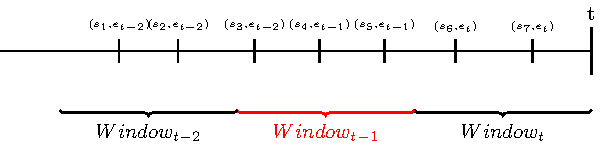
\includegraphics{tikz/window.pdf}
        \end{center}
    \end{figure}
    
    The sampling window then advances every $x$ seconds, setting the new window: 
    \begin{center}
        From: $(t-1)_l$, $(t-1)_u$ $\xrightarrow{t + 1}$ $t_l, t_u$. \\
        Where: $t_l = (t-1)_u$ and $t_u = (t-1)_u + x$ 
    \end{center}
    
    The $\Delta$Qs which are observed and calculated in a sampling window are not precise, this is why we need to introduce the polling window.

    \subsection{Polling window (Observing multiple $\Delta$Qs over a time interval)}
        The polling window is the window of $\Delta$Qs which are stored to keep a snapshot of the system over time and over which confidence bounds are calculated. The polling window serves to improve the precision of the $\Delta$Q measurement.
        
        Suppose we are at time $t = 0$, the polling window will have 0 $\Delta$Qs. As the sampling window advances, more $\Delta$Qs are sampled, which in turn are added to the snapshot and to the confidence bounds.

        The limit of $\Delta$Qs for a polling window (subsequently snapshots and confidence bounds) is 30 $\Delta$Qs. At $t= 31$, the older $\Delta$Qs will be removed from the polling window and in turn from the snapshots and confidence bounds. Newer sampled $\Delta$Qs will be added, keeping the limit of $\Delta$Qs in a polling window to 30.

 
    \section{Triggers}
    Much like an oscilloscope that has a trigger mechanism to capture periodic signals or investigate a transient event \cite{osc-t}, the \textit{$\Delta$Q oscilloscope} has a similar mechanism that can recognise when an observed $\Delta$Q violates certain conditions regarding required behaviour and record snapshots of the system.

    Each time an observed $\Delta$Q is calculated, it is checked against the requirements set by the user. If these requirements are not met, a trigger is fired and a snapshot of the system is saved to be shown to the user. 
    
    \subsection{Snapshot}
    A snapshot of the system gives insights into the system before and after a trigger was fired. It gives the user a still of the system, as if it was frozen in time. All the $\Delta$Qs which are calculated during the system's execution are stored away. Then, if no trigger is fired, older $\Delta$Qs are removed. Otherwise, the oscilloscope keeps recording $\Delta$Qs without removing older ones, to allow the user to look at the state of the system before and after the trigger.
    


   % \chapter{An overview of $\Delta$Q}
    \section{Timeliness}
    \section{Outcome}

    \section{Quality attenuation}
    \section{Convolution}
    \section{Operators}
        \subsection{First to finish}
        \subsection{All to finish}
        \subsection{Probabilistic choice}
    
    \section{Outcome diagram}


    \chapter{Oscilloscope: User level concepts}
    The following chapter gives insights on the user level concepts of $\Delta$QSD in the oscilloscope. They are the concepts needed by the user to understand how the oscilloscope works.
    \begin{itemize}
        \item We first provide insights into how $\Delta$QSD was implemented in the oscilloscope, the parameters that define a probe's $\Delta$Q, its representation and what can be done with $\Delta$Qs. We show how probe's $\Delta$Q(s) will be shown in the oscilloscope.
        \item We then provide a language to write outcome diagrams based on an already existing syntax.
        \item Lastly, we explain the different controls present on the oscilloscope dashboard.
    \end{itemize}

\section{$\Delta$Q implementation}

Originally, $\Delta$Q(x) denotes the probability that an outcome occurs in a time $t \le x$, defining then the "intangible mass" of such IRV as $1 - \lim_{x\to\infty} \Delta Q (x)$.
We then extend the original definition to fit real time constraints, needing to calculate $\Delta$Qs continuously.

For a given observable, $\Delta$Q($t_l$, $t_u$, $dMax$) is the probability that the time of series with samples between time $t_l < t_u$, an observable occurs in time t $\le$ dMax.


\subsection{Internal representation of a $\Delta$Q}
    We provide a $\Delta$Q class to calculate the $\Delta$Q of an observable between a lower time bound $t_l$ and an upper time bound $t_u$.
    The $\Delta$Q can be calculated in various ways: \\
    The first way is by having $n$ collected samples between $t_l$ and $t_u$ and calculating its PDF and then calculating the \textit{empirical cumulative distribution function} (ECDF) based on its PDF.
    A $\Delta$Q can also be calculated by performing operations on two or more $\Delta$Qs, the notion of samples is then lost between calculations, as the interest shifts towards the calculate PDFs and ECDFs.
    Below, is how both are calculated given $n$ samples.
    \subsubsection{PDF}
  We approximate the PDF of the observed random variable $\textbf{X}$ via a histogram. We partition the values into $N$ bins of equal width, this is required to ease future calculations.
        Given $\lbrack x_i, x_{i+1} \rbrack$ the interval of a bin $i$, where $x_i = i\Delta x$, and $\hat{p}(x_i)$ the value of the PDF at bin $i$, for $n$ bins:
        \begin{equation}
            \begin{cases}
                \hat{p}(i) = \dfrac{n_i}{n}, \text{if } i \le n \\
                \hat{p}(i) = \hat{p}(n), \text{if } i > n \\
            \end{cases}
            \label{eq:pdf}
        \end{equation}
   With $n_i$ the number of successful samples whose elapsed time is contained in the bin $i$, $n$ the total number of samples.
    \subsubsection{ECDF}
    The value $\hat{f}(x_i)$ of the ECDF at bin $i$ with $n$ bins can be calculated as:
    \begin{equation}
        \begin{cases}
            \hat{f}(i) = \sum_{j=1}^{i} \hat{p}(j), & \text{if } i \le n \\  
            \hat{f}(i) = \hat{f}(x_n), & \text{if } i > n 
        \end{cases}
        \label{eq:cdf}
    \end{equation}
    
    \subsection{dMax}
        The key concept of $\Delta$QSD is having a maximum delay after which we consider that the execution is failed, this is represented in an observable as $dMax$. The user defines, for each observable the maximum delay its execution can have. \\ 
Setting a maximum delay for an observable is not a job that can be done one-off and blindly, it is something that is done with an underlying knowledge of the system inner-workings and must be thoroughly fine tuned during the execution of the system by observing the resulting distributions of the obtained $\Delta$Qs. \\

We define in our oscilloscope a formula to dynamically define a maximum delay based on the formula:
\begin{equation}
    dMax = \Delta_{t base} * 2^n * N  
    \label{eq:dMax}
\end{equation}
Where:
\begin{itemize}
    \item $\Delta_{t base}$ represents the base width of a bin, equal to 1ms.
    \item $N$ the number of bins.
\end{itemize}

Some tradeoffs must though be acknowledged when setting these parameters, a higher number of bins corresponds to a higher number of calculations and space complexity, a lower $dMax$ may correspond to more failures. These are all tradeoffs that must be considered by the system engineer and set accordingly.
    \begin{figure}[H]
        \begin{center}
            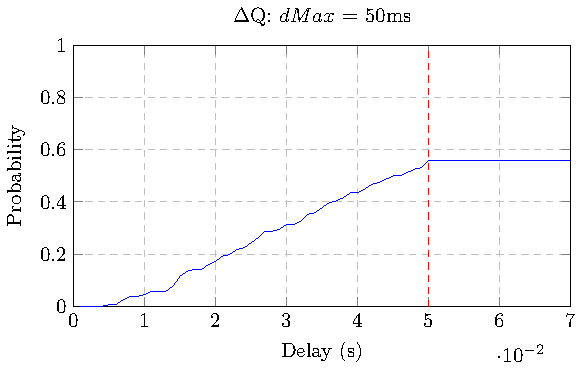
\includegraphics[width=\textwidth, scale = 0.6]{tikz/cdf_dmax.pdf}
        \end{center}
        \caption{$\Delta$Q: $dMax$ = 50ms, the CDF will stay constant when delay $> dMax$}
    \end{figure}

    \subsection{QTA}
        A simplified QTA is defined for observables. We define 4 points for the step function at 25, 50, 75 percentile and the maximum amount of failures accepted for an observable. An observed $\Delta$Q will calculate that based on the samples collected. 
\subsection{Operations}
    In a previous section [REF HERE] we talked about the possible operations that can be performed on and between $\Delta$Qs, the time complexity of FTF, ATF and PC is trivially $\mathcal{O}(N)$ where N is the number of bins. As to convolution, the naïve way of calculating convolution has a time complexity of $\mathcal{O}(N^2)$, this quickly becomes a problem as soon as the user wants to have a more fine-grained understanding of a component. Below we present two ways to perform convolution.

        \subsubsection{Convolution}
        
        \paragraph{Naïve convolution}
        Given two $\Delta$Q binned PDFs $f$ and $g$, the result of the convolution $f \circledast g$ is given by 
        \begin{equation}
            (f \circledast g)\lbrack n \rbrack = \sum_{m = 0}^{N} = f\lbrack m \rbrack g \lbrack n - m \rbrack  
            \label{eq:discconv}
        \end{equation}
            

    \paragraph{Fast Fourier Transform Convolution}
        FFTW (Fastest Fourier Transform in the West) is a C subroutine library [cite site] for computing the discrete Fourier Transform in one or more dimensions, of arbitrary input size, and of both real and complex data. We use FFTW in our program to compute the convolution of $\Delta$Qs.
    Whilst the previous algorithm is far too slow to handle a high number of bins, convolution leveraging Fast Fourier Transform (FFT) allows us to reduce the amount of calculations to $\mathcal{O}(n \text{log} n)$. \\
    FFT and naïve convolution produce the same results in our program barring $\varepsilon$ differences (around $10^{-18}$) in bins whose result should be 0.

    \subsubsection{Arithmetical operations}
        We can apply a set of arithmetical operations between $\Delta$Qs ECDFs, and on a $\Delta$Q.
    \paragraph{Scaling (multiplication)} A $\Delta$Q can be scaled w.r.t a constant $0 \le j \le 1$. It is equal to binwise multiplication on ECDF bins.
    \begin{equation}
        \hat{f_r}(i) = \hat{f}(i) \cdot j
        \label{eq:mul_ecdf}
    \end{equation}

    \paragraph{Operations between $\Delta$Qs} 
        Addition, subtraction and multiplication can be done between two $\Delta$Q of equal bin width (but not forcibly of equal length) by calculating the operation between the two ECDFs of the $\Delta$Qs:
        \begin{equation}
            \Delta \text{Q}_{AB}(i) = \hat{f_A}(i) [\cdot, +, -] \hat{f_B}(i)
            \label{eq:op_dq}
        \end{equation}
    \subsection{Confidence bounds}
    To observe the stationarity of a system we must observe a window of $\Delta$Qs of an observable and calculate confidence bounds over said windows. We present here the formulae required to give such bounds with 95\% confidence level. \\
        For a bin $i$, its mean over a window is:
            \begin{equation}
                \mu_i = \dfrac{1}{n_i} \sum_{j=1}^{n_i} x_{ij}
                \label{eq:mean_ecdf}
            \end{equation}
        Where $x_{ij}$ is a bin's $i$ value for an ECDF $j$.
        Its variance:
            \begin{equation}
                \sigma^2_i = \dfrac{1}{n_i} \sum_{j=1}^{n_i} x^2_{ij} - \mu^2_i
                \label{eq:var_ecdf}
            \end{equation}
        The confidence intervals $CI_i$ for a bin $i$ can then be calculated as:
        \begin{equation}
            CI_i = \mu_i \pm z_{\alpha/2} \cdot \dfrac{\sigma_i}{\sqrt{n_i}}      
            \label{eq:ci_i}
        \end{equation}
    The bounds can be updated dynamically by inserting or removing a $\Delta$Q, this allows us to consider a small window of execution rather than observing the whole execution.

    \subsection{Rebinning}
        Rebinning refers to the aggregation of multiple bins of a bin width $i$ to another bin width $j$. \\  
        Operations between $\Delta$Qs can be done on $\Delta$Qs that have the same bin width, this is why it is fundamental that all observables have a common $\Delta_{tbase}$. This allows for fast rebinning to a common bin width. \\
        Given two $\Delta$Qs $\Delta$Q$_i$, $\Delta$Q$_j$:
        \begin{center}
            $\Delta_{Tij}$ = max \{$\Delta_{Ti}, \Delta_{Tj} \}$
        \end{center}
        and the PDF of the rebinned $\Delta$Q at bin $b$, from the original PDF of $n$ bins, where $k$ = $\frac{\Delta{_Ti}}{\Delta_{Tj}}$:
        \begin{equation}
            p'_b = \sum_{n=b \cdot k}^{b+ 1 \cdot k - 1} p_n, \quad b=0,1,\dots \lceil \frac{N}{k} \rceil  
        \end{equation}
        We perform rebinning to a higher bin width for a simple reason, while this leads to loss of information for the bin with the lowest bin width, rebinning to a lower bin width would imply inventing new values for the $\Delta$Q with the highest bin width.
       
        
        \begin{figure}[H]
            \begin{center}
                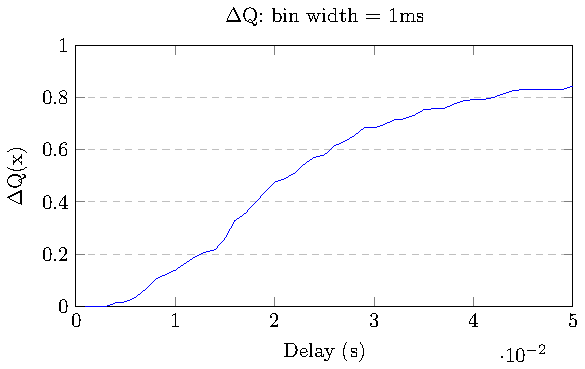
\includegraphics[width=\textwidth]{tikz/cdf.pdf}
            \end{center}
            \caption{Sample $\Delta$Q with 1ms bins}
        \end{figure}

 
        \begin{figure}[H]
            \begin{center}
                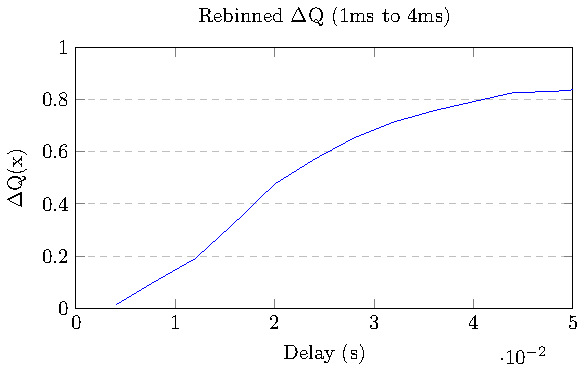
\includegraphics[width=\textwidth]{tikz/rebinned_cdf.pdf}
            \end{center}
            \caption{Previous $\Delta$Q after rebinning to 4ms bins}
        \end{figure}

\section{$\Delta$Q display}
    An observable's displayed graph must contain the following functions:
    \begin{itemize}
        \item The mean and confidence bounds of a window of previous $\Delta$Qs
        \item The observed $\Delta$Q($t_l, t_u, dMax$)
        \item For a probe, the calculated $\Delta$Q from its components.
        \item Its QTA
    \end{itemize}
    This allows for the user to observe if a $\Delta$Q has deviated from normal execution, analyse its stationarity, nonlinearity and observe its execution.
    \begin{figure}[!ht]    
    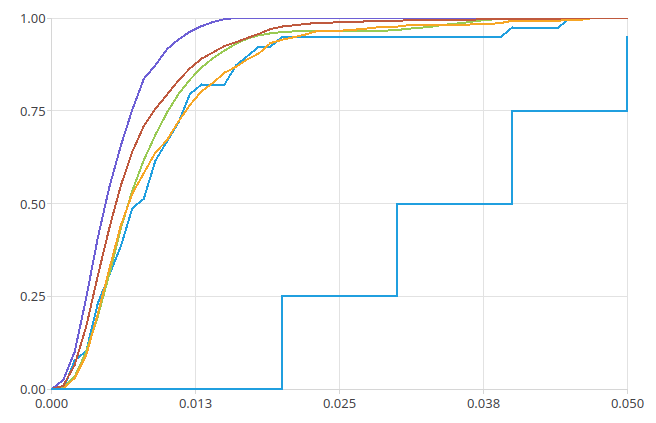
\includegraphics[scale =0.8, width=\textwidth]{img/dqdispl.png}
    \end{figure}

  \section{Outcome diagram}
        An abstract syntax for outcome expressions and consequently outcome diagrams has already been defined in a previous paper \cite{art}, nevertheless, the oscilloscope provides additional features not included in the original syntax and, moreover, needs a textual way to define an outcome diagram. 
       
        We define thus a grammar to create an outcome diagram in our oscilloscope, our grammar is a textual interpretation of the abstract syntax.
        \subsection{Probes}
            To attach probes in the oscilloscope, the user must define outcomes and probes that observe outcome expressions.
            \subsubsection{Outcome}
                In our system an outcome is defined with its name
                \begin{minted}{text}
                    ... = outcomeName;
                \end{minted}
        
        \subsubsection{Probes containing outcome expressions}
            A probe can contain one component or a sequence of causally linked components.
            The user can define as many probes that contain outcome expressions as they want, they have to be declared as follows:
            \begin{minted}{text}
                probe = component [-> component2];
                probe2 = newComponent -> anotherComponent;
            \end{minted}
    
            These probes can be reused in other probes or in the system by adding \texttt{"s:"} (subsystem) before they are used.
            \begin{minted}{text}
                probe3 = s:probe -> s:probe2;
            \end{minted}
 
        \subsection{Operators, outcome expressions}
            To build a system, we must define the relations between outcomes and outcome expressions, below is how they can be defined. 

            First-to-finish, all-to-finish and probabilistic choice must contain at least two components, this is because the operations to calculate the \textit{calculated} $\Delta$Q rely on using the CDF of the components that define the operator.
            
        \subsubsection{Causal link}
            A causal link between two components can be defined by a right arrow from \texttt{component\_i} to \texttt{component\_j}
        \begin{minted}{text}
            component_i -> component_j 
        \end{minted}
        
        \subsubsection{All-to-finish operator}
            An all-to-finish operator needs to be defined as follows:
            \begin{minted}{text}
                a:name(component1, component2...)
            \end{minted}

        \subsubsection{First-to-finish operator}
            A first-to-finish operator needs to be defined as follows.
            \begin{minted}{text}
                f:name(component1, component2...)
            \end{minted} 

        \subsubsection{Probabilistic choice operator}
            A probabilistic choice operator needs to be defined as follows:
            \begin{minted}{text}
                p:name[probability_1, probability_2, ... probability_i](component_1, component_2, ..., component_i) 
            \end{minted}
            In addition to being comma separated, the number of probabilities inside the brackets must match the number of components inside the parentheses. For $n$ probabilites $p_i$, $0 < p_i < 1$, $\sum_{i = 0}^{n} p_i = 1$ 
        
            
        \subsection{Limitations}
            Our system has a few limitations compared to the theoretical applications of $\Delta$Q, namely, no cycles are allowed in the definition of a system.
        
        \begin{minted}{text}
            probe = s:probe_2;
            probe_2 = s:probe;
        \end{minted}
        The above example is not allowed and will raise an error when defined.  



\section{Dashboard}
    The dashboard is devised of multiple sections where the user can interact with the oscilloscope, create the system, observe the behaviour of its components, set triggers.

    \subsection{Sidebar}
        The sidebar has multiple tabs, we explain here the responsibility of each one.

    \subsubsection{System/Handle plots tab}

    \paragraph{System creation}
        In this tab the user can create its system using the grammar defined before, he can save the text he used to define the system or load it, the system is saved to a file with any extension, we nevertheless define an extension to save the system to, the extension \texttt{.dq}.
        If the definition of the input is wrong, he will be warned with a pop up giving the error the parser generator encountered in the creation of a system.

    \paragraph{Adding a plot}
        Once the system is defined, the user can choose the probes he wants to plot. They can select multiple probes per plot and display multiple plots on the oscilloscope window.
    
    \paragraph{Polling rate}
        The user can choose the polling rate of the system: How often $\Delta$Qs are calculated and displayed in the oscilloscope.

    \paragraph{Editing a plot}
        By clicking onto a plot that is being shown, the user can choose to add or remove probes to and from it. Multiple probes can be selected to either be removed or added.

    \subsubsection{Parameters tab}
        In this tab, the user can define parameters for the probes they have defined.

    \paragraph{Set a QTA}
        The user is given the choice to set a QTA for a given observable, they have 4 fields where they can fill in which correspond to the percentiles and the maximum amount of failures allowed, they can change this dynamically during execution.

    \paragraph{dMax, bins}
        The user has a slider which goes from -10 to 10, where they can set the parameters we explained previously, $n$, the exponent of $\Delta_{tbase} \cdot 2^n$ and the bins $N$. When these informations are saved by the user, the new $dMax$ is transmitted to the stub and saved for the selected observable.

    \subsubsection{Triggers tab}
        In the triggers tab the user can set triggers and observe the snapshots of the system.

    \paragraph{Set triggers}
        The user can set which triggers to fire for the probes they desire, they are given checkboxes to decide which ones to set as active or not (by default, the triggers are deactivated).
    
    \paragraph{Fired triggers}
        Once a trigger is fired, the system start a timer, during which all probes start recording the observed $\Delta$Qs (and the calculated ones if applicable) without discarding older ones. Once the timer expires, the snapshot is saved for the user in the triggers tab. In the dashboard, it indicates when the trigger was fired (timestamp) and the name of the probe which fired it.
    
    \subsection{Plots window}
        To the left, the main window shows the plots of the probes being updated in real time. 

    \subsection{Stub controls}
        Below the sidebar, two buttons are present, these buttons communicate to the stub. 
         
        The \textbf{start stub} button sends a message to the stub, telling it to start sending spans. The \textbf{stop stub} button stops it.

\section{Triggers}
    Like an oscilloscope that has a trigger mechanism that fires when a signal of interest is recognized by the oscilloscope, our $\Delta$Q oscilloscope has a similar mechanism of triggers that are fired when an observed $\Delta$Q violates certain conditions. Let us define what these triggers are.

    \subsection{Load}
        A trigger on an observed $\Delta$Q can be fired if 
    \begin{center}
        nSamples($\Delta$Q($t_l, t_u, dMax$)) > maxAllowedSamples 
    \end{center}

    \subsection{QTA}
        There are two possible [can change] triggers that can be fired based on the observable defined $\Delta$Q's QTA.   
        \subsubsection{Percentiles}
            A trigger can be fired if:
        \begin{center}
            $\Delta$Q$_{obs}$[percentile] $<$ observableQTA$_{req}$[percentile] \quad $\forall \text{ percentile } \{0.25, 0.5, 0.72\}$
        \end{center}
        \subsubsection{Failure}
            A trigger can be fired on the percentage of failed samples for $\Delta$Q($t_l, t_u, dMax$) if:
        \begin{center}
            success($\Delta$Q$_{obs}$) $<$ success(observableQTA$_{req}$)
        \end{center}

    \subsection{Time series snapshots}
        When a trigger is fired, the oscilloscope will capture ...



    \chapter{Oscilloscope: implementation}
    The following chapter gives a more technical description of the internals of the oscilloscope.
    \begin{itemize} 
        \item We provide a more in-depth look at the $\Delta$QSD concepts introduced in the previous chapter.
        \item We then explain how the $\Delta$Q adapter works, its API and the underlying mechanism that let us export outcome instances to the oscilloscope.
        \item Next we give a technical explanation of the parser generator we used to parse the outcome diagram syntax.
        \item Lastly, we briefly talk about the dashboard graphical framework.
    \end{itemize}

    \section{$\Delta$QSD implementation}
    A probe's $\Delta$Q can be represented internally by a PDF and displayed as an CDF. Here is how both can be calculated given $n$ outcome instances.
    
    \subsection{Histogram representation}
        The $\Delta$Q representation is one of a histogram for its PDF and a cumulative histogram for its CDF.
    \subsubsection{PDF}
  We approximate the PDF of the observed $\Delta$Q via a histogram. We partition the values into $N$ bins of equal width, Given $\lbrack x_i, x_{i+1} \rbrack$ the interval of a bin $i$, where $x_i = i\Delta t$, and $\hat{p}(x_i)$ the value of the PDF at bin $i$, for $n$ bins:
        \begin{equation}
            \begin{cases}
                \hat{p}(i) = \dfrac{s_i}{n}, \text{if } i \le n \\
                \hat{p}(i) = 0, \text{if } i > n \\
            \end{cases}
            \label{eq:pdf}
        \end{equation}
    Where $s_i$ the number of successful outcome instances whose elapsed time is contained in the bin $i$, $n$ the total number of instances. \cite{stat}

    \subsubsection{CDF}
        The value $x_i = \hat{f}(i)$ of the CDF at bin $i$ with $n$ bins can be calculated as:
        \begin{equation}
            \begin{cases}
                \hat{f}(i) = \sum_{j=1}^{i} \hat{p}(j), & \text{if } i \le n \\  
                \hat{f}(i) = \hat{f}(n), & \text{if } i > n 
            \end{cases}
            \label{eq:cdf}
        \end{equation}
 
    \begin{figure}[H]
            \begin{center}
                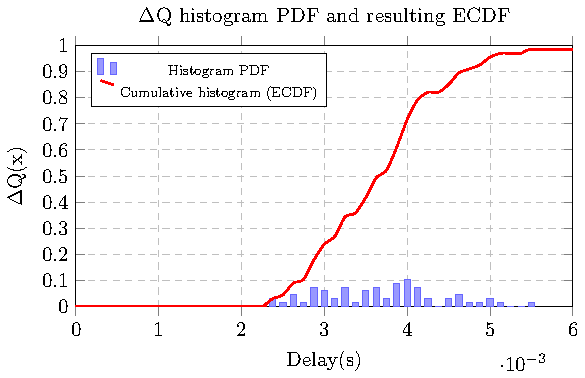
\includegraphics[scale=1]{tikz/pdf_dq.pdf} 
            \end{center}
            \caption{Blue bins: PDF of a sample $\Delta$Q. Red: Resulting CDF of $\Delta$Q PDF, the CDF is what is displayed on the dashboard.}
        \end{figure}

    \subsection{dMax}
        We introduced $dMax$ in the previous chapters, we provide here the full equation that allows $dMax$ to be calculated:
        \begin{equation}
            dMax = \Delta t_{base} * 2^n * N  
            \label{eq:dMaxU}
        \end{equation}
        Where:
        \begin{itemize}
            \item $\Delta t_{base}$ represents the base width of a bin, equal to 1ms.
            \item $n$ the exponent that is set by the user in the dashboard. It is limited to [-10, 10].
            \item $N$ the number of bins.
        \end{itemize}
            We chose 1 ms in combination with $2^n$ as it allows us to go from very fine bin widths ($\approx$ 1 $\mu$) to large bin widths ($\approx$ 1 s) 
    \subsection{Convolution} \label{convol}
    We present the two solution to perform convolutions we explored during the implementation.  
        \subsubsection{Naïve convolution}
        Given two $\Delta$Q binned PDFs $f$ and $g$ with equal bin widths, the result of the convolution $f \circledast g$ is given by \cite{conv}: 
        \begin{equation}
            (f \circledast g)\lbrack n \rbrack = \sum_{m = 0}^{N} = f\lbrack m \rbrack g \lbrack n - m \rbrack  
            \label{eq:discconv}
        \end{equation}

        The naïve way of calculating convolution has a time complexity of $\mathcal{O}(N^2)$, this quickly becomes a problem as soon as the user wants to have a more fine-grained understanding of a component. Moreover, the oscilloscope started presenting noticeable lag and frame skipping. This is why we decided to explore Fast Fourier Transform convolution. 
 
    \subsubsection{Fast Fourier Transform Convolution}
        FFTW (Fastest Fourier Transform in the West) is a C subroutine library \cite{fftw3} for computing the discrete Fourier Transform in one or more dimensions, of arbitrary input size, and of both real and complex data. We use FFTW in our program to compute the convolution of $\Delta$Qs. We adapt our script from an already existing one found on GitHub. \cite{fft}
    
    Whilst the previous algorithm is far too slow to handle a high number of bins, convolution leveraging Fast Fourier Transform (FFT) allows us to reduce the amount of calculations to $\mathcal{O}(N \text{log} N)$. This is why the naïve convolution algorithm is not used. We will analyse the time gains in a later chapter.
    
    FFT and naïve convolution produce the same results in our program, barring $\varepsilon$ differences (around $10^{-18}$) in bins whose result should be 0. This is most likely due to rounding error.
    
    FFTs algorithms are plenty, the choice of the one to use is left up to the subroutine via the parameter \texttt{FFTW\_ESTIMATE} \cite{fft-h}.

    \subsection{Arithmetical operations}
        The FTF, ATF and PC operators on $\Delta$Qs use a simple set of arithmetical operations to calculate a $\Delta$Q.   
    The time complexity of FTF, ATF and PC is trivially $\mathcal{O}(N)$ where N is the number of bins.
 
    \paragraph{Scaling (multiplication)} A $\Delta$Q can be scaled w.r.t. a constant $0 \le j \le 1$. It is equal to binwise multiplication on CDF bins. It is used for the probabilistic choice operator.
    \begin{equation}
        \hat{f_r}(i) = \hat{f}(i) \cdot j
        \label{eq:mul_ecdf}
    \end{equation}

    \paragraph{Operations between $\Delta$Qs} 
        Addition, subtraction and multiplication can be done between two $\Delta$Q of equal bin width (but not forcibly of equal length) by calculating the operation between the two CDFs of the $\Delta$Qs:
        \begin{equation}
            \Delta \text{Q}_{AB}(i) = \hat{f_A}(i) [\cdot, +, -] \hat{f_B}(i)
            \label{eq:op_dq}
        \end{equation}
    They are used for all operators.

    \subsection{Confidence bounds}
        Here is how we calculate the mean and lower/upper confidence for the $\Delta$Qs CDF at bin $i \quad \forall i < N$. \cite{stat}

        For $x_{ij}$ the value of an CDF $j$ at bin $i$, the mean of all CDFs for the bin over a window is:
            \begin{equation}
                \mu_i = \dfrac{1}{n_i} \sum_{j=1}^{n_i} x_{ij}
                \label{eq:mean_ecdf}
            \end{equation}
        Its variance:
            \begin{equation}
                \sigma^2_i = \dfrac{1}{n_i} \sum_{j=1}^{n_i} x^2_{ij} - \mu^2_i
                \label{eq:var_ecdf}
            \end{equation}
        The confidence intervals $CI_i$ for a bin $i$ can then be calculated as:
        \begin{equation}
            CI_i = \mu_i \pm \dfrac{\sigma_i}{\sqrt{n_i}}      
            \label{eq:ci_i}
        \end{equation}

        \subsection{Rebinning}
            Rebinning refers to the aggregation of multiple bins of a bin width $i$ to another bin width $j$. 
            Previous operations between $\Delta$Qs must be done on $\Delta$Qs that have the same bin width. This is why it is fundamental that all probes have a common $\Delta t_{base}$ and why we have a $2^n$ factor to calculate the total bin width.

            Given two $\Delta$Qs $\Delta$Q$_i$, $\Delta$Q$_j$, the common bin width $\Delta t_{ij}$ is:
            \begin{center}
                $\Delta t_{ij}$ = max \{$\Delta_{Ti}, \Delta_{Tj} \}$
            \end{center}
            and the PDF of the rebinned $\Delta$Q at bin $b$, from the original PDF of $n$ bins, where $k$ = $\frac{\Delta{_Ti}}{\Delta_{Tj}}$:
            \begin{equation}
                p'_b = \sum_{n=b \cdot k}^{b+ 1 \cdot k - 1} p_n, \quad b=0,1,\dots \lceil \frac{N}{k} \rceil  
            \end{equation}
            We perform rebinning to a higher bin width for a simple reason. While this leads to loss of information for the $\Delta$Q with the lowest bin width, rebinning to a lower bin width would imply inventing new values for the $\Delta$Q with the highest bin width.
        \begin{figure}[H]
            \centering
            \begin{subfigure}{.5\textwidth}
                \centering
                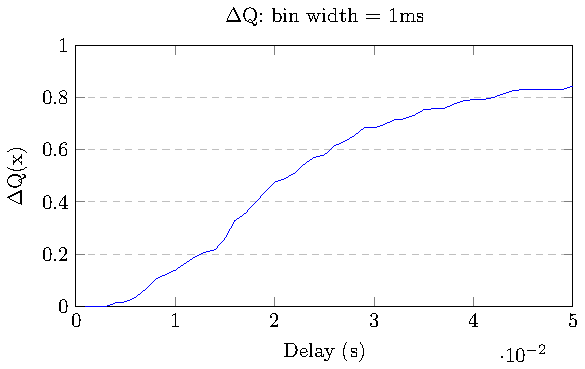
\includegraphics[width =0.98\textwidth]{tikz/cdf.pdf}
                \label{fig:nrb}
                \subcaption{Sample $\Delta$Q with 1ms bins}%
            \end{subfigure}%
            \begin{subfigure}{.5\textwidth}%
                \centering%
                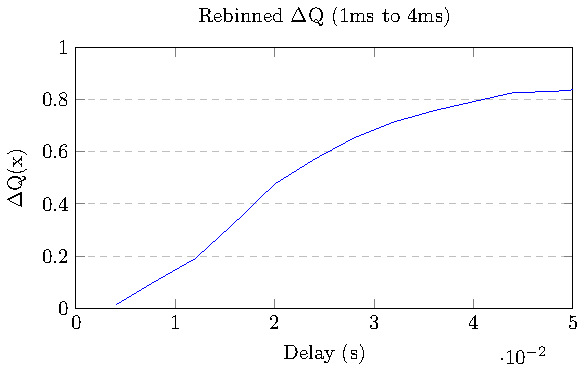
\includegraphics[width =0.98\textwidth]{tikz/rebinned_cdf.pdf}%
                \label{fig:sub2}%
                \subcaption{$\Delta$Q on the left after rebinning to 4ms bins}%
            \end{subfigure}%
            \label{fig:w1w2hb}%
            \end{figure}%



    \section{Adapter}
    The adapter, called \texttt{dqsd\_otel} is a rebar3 \cite{rebar3} application built to replace OpenTelemetry calls and create outcome instances, it is designed to be paired with the oscilloscope to observe an Erlang application.
    
    \subsection{API}
        The adapter functions to be used by the user are made to replace OpenTelemetry calls to macros as for \texttt{?start\_span} and \texttt{?with\_span} and \texttt{?end\_span}. This is to make the adapter less of an encumbrance for the user. 

        Moreover, the adapter will always start OpenTelemetry spans but only start outcome instances if the adapter has been activated. The adapter can be activated by the oscilloscope by pressing the "start adapter" button and can be stopped via the "stop adapter" button.
         
        \subsubsection{start\_span/1, start\_span/2}
        
        \begin{minted}{erlang}        
start_span/1: -spec start_span(binary()) -> {opentelemetry:span_ctx(), pid() | ignore}.
start_span/2: -spec start_span(binary(), map()) -> {opentelemetry:span_ctx(), pid() | ignore}.  
        \end{minted}
        
        \paragraph{Parameters:}
        \begin{itemize}
            \item Name: Binary name of the probe.
            \item Attributes: The OpenTelemetry span attributes (Only for start\_span/2).
        \end{itemize} 
        
        \texttt{start\_span} incorporates OpenTelemetry \texttt{?start\_span(Name)} macro.
        
        \paragraph{Return:} 
        The function returns either:
        \begin{itemize}
            \item  \texttt{\{SpanCtx, span\_process\_PID\}} if the adapter is active and the probe's $dMax$ has been set.
            \item \texttt{\{SpanCtx, ignore\}} if one of the two previous conditions was not respected.
        \end{itemize}
        With SpanCtx being the context of the span created by OpenTelemetry.
        
        \subsubsection{with\_span/1, with\_span/2}
        
        \begin{minted}{erlang}
with_span/1: -spec with_span(binary(), fun(() -> any())) -> any().
with_span/2: -spec with_span(binary(), map(), fun(() -> any())) -> any().
        \end{minted}
         
        \paragraph{Parameters:}
            \begin{itemize}
                \item Name: Binary name of the probe.
                \item Fun: Zero-arity function representing the code of block that should run inside the \texttt{?with\_span} macro.
                \item Attributes: The OpenTelemetry span attributes (Only for with\_span/3).

            \end{itemize}

        \texttt{with\_span} incorporates OpenTelemetry \texttt{with\_span} macro. \\
        \paragraph{Return:}
            \texttt{with\_span} returns what \texttt{Fun} returns (\texttt{any()}).
        
        \subsubsection{end\_span}
            \begin{minted}{erlang}                
-spec end_span(opentelemetry:span_ctx(), pid() | ignore) -> ok | term().
            \end{minted}
            \paragraph{Parameters:}
            \begin{itemize}
                \item SpanCtx: The context of the span returned by \texttt{start\_span}.
                \item Pid: \texttt{span\_process\_PID} || \texttt{ignore}.
            \end{itemize}

    As is the case for \texttt{start\_span}, \texttt{end\_span} incorporates an OpenTelemetry macro, in this case \texttt{?end\_span(Ctx)}. \\

        \subsubsection{fail\_span}
        \begin{minted}{erlang}        
-spec fail_span( pid() | ignore) -> ok | term().
        \end{minted}
        \paragraph{Parameter:}
             \begin{itemize}
                \item Pid: \texttt{ignore} || \texttt{span\_process\_PID}.
            \end{itemize}
            \texttt{fail\_span} does not incorporate any OpenTelemetry macro, it is let up to the user to decide how to handle failures in execution. \\
        

        \subsubsection{span\_process}
            \texttt{span\_process} is the process, spawned by \texttt{start\_span}, responsible for handling the \texttt{end\_span, fail\_span, timeout} messages.

            Upon being spawned, the process starts a timer with time equal to the $dMax$ set by an user for the probe being observed, thanks to \texttt{erlang:send\_after}. When the timer runs out, it sends a \texttt{timeout} message to the process.
        
        The process can receive three kinds of messages:
        \begin{itemize}
            \item \texttt{\{end\_span, end\_time\}}: This will send a custom span to the oscilloscope with the start and end time of the execution of the probe.
            \item \texttt{\{fail\_span, end\_time\}}: This will send a custom span to the oscilloscope indicating that an execution of a probe has failed.
            \item \texttt{\{timeout, end\_time(StartTime + $dMax$)\}}: If the program hasn't ended the span before $dMax$, the timer will send a \texttt{timeout} message and it will send an outcome instance to the oscilloscope indicating that an execution of a probe has timed out.
        \end{itemize}
        The process is able to receive one and only message, if the execution times out and subsequently the span is ended, the oscilloscope will not be notified as the process is defunct. This is assured by Erlang documentation:
        \begin{center}
            \textit{If the message signal was sent using a process alias that is no longer active, the message signal will be dropped.} \cite{erl-s}
        \end{center}

    \subsection{Handling outcome instances}
        To create outcome instances of a probe we must obtain three important informations:
        \begin{itemize}
            \item Its name.
            \item The time when the span was started.
            \item Its $dMax$.
        \end{itemize}
        
        They start time and end time are supplied by calling this function:
        \begin{minted}{erlang}
        StartTime/EndTime = erlang:system_time(nanosecond).
        \end{minted}
        The name is given when starting a span and the $dMax$ is stored in a dictionary in the adapter. 

            The outcome instance is created only if two conditions are met: the adapter has been set as active and the user set a timeout for the probe, the functions will spawn a \texttt{span\_process} process, passing along all the necessary informations. \\
        Once the span is subsequently ended/timed out/failed, the function \texttt{send\_span} creates a message carrying all the informations and sends it to the C++ server. The formatting of the messages is the following:
        \begin{minted}{text}
            n:Observed name, b: Start time (beginning), e: End time (end or deadline), s: The status
        \end{minted}

    \subsection{TCP connection}
        The adapter is composed of two \texttt{gen\_server} which handle communication to and from the oscilloscope. This gen\_server behaviour allows the adapter to send spans asynchronously to the oscilloscope.

        \subsubsection{TCP server}
            The TCP server is responsible for receiving commands from the oscilloscope. It can be run by setting its IP and port via:
            \begin{minted}{erlang}
                -spec start_server(string() | binary() | tuple(), integer()) -> ok | {error, Reason}
            \end{minted}
            The oscilloscope can send commands to the adapter, these commands are:
            \begin{itemize}
                \item \texttt{start\_stub}: This command sets the adapter as active, it can now send outcome instances to the oscilloscope if the probe's $dMax$s are defined.
                \item \texttt{stop\_stub}: This commands sets the adapter as inactive, it will no longer send outcome instances to the oscilloscope.
                \item \texttt{set\_timeout;probeName;timeout}: This command indicates to the adapter to set the $dMax = \text{timeout}$ for a probe, a limit of the adapter is that erlang:send\_after does not accept floats as timeouts, so the timeout will be rounded to the nearest integer.
            \end{itemize}

        \subsubsection{TCP client}
            The TCP client allows the adapter to send the spans to the oscilloscope.
            The client connects over TCP to the oscilloscope by connecting to the oscilloscope server's address and opens a socket where it can send the outcome instances.
            \begin{minted}{erlang}
                -spec try_connect(string() | binary(), integer()) -> ok.
            \end{minted}

    \section{Parser}
        To parse the system, we use the C++ ANTLR4 (ANother Tool for Language Recognition) library \cite{antlr4}. 
        \subsection{ANTLR}
    According to ANTLR website \cite{antlr4}: 
    \begin{quote}
        ANTLR is a parser generator for reading, processing, executing or translating structured text files. ANTLR generates a parser that can build and walk parse trees.
    \end{quote}

 ANTLR is just one of the many parsers generators available in C++ (flex/bison \cite{flexb}, lex/yacc \cite{lexy}). Although it presents certain limitations, its generated code is simpler to handle and less convoluted with respect to the other possibilities.

        ANTLR uses Adaptive LL(*) \textit{(ALL(*))} parser, namely, it will ``move grammar analysis to parse-time, without the use of static grammar analysis''. \cite{antlr}

        \subsection{Grammar}
            ANTLR provides a yacc-like metalanguage \cite{antlr} to write grammars. The grammar we have written can be found in the appendix \ref{code:grammar}.
              
    \subsubsection{Limitations}
        A previous version was implemented in Lark \cite{lark}, a python parsing toolkit. The python version was quickly discarded due to a more complicated integration between Python and C++. Lark provided Earley(SPPF) strategy which allowed for ambiguities to be resolved, which is not possible in ANTLR. \\
        For example the following system definition presents a few errors:
        \begin{minted}{text}
        probe = s -> a -> f -> p;
        \end{minted}
    While Lark could correctly guess that everything inside was an outcome, ANTLR expects \texttt{``:''} after ``s, a, f'' and ``p'', thus, one can not name an outcome by these characters, as the parser generator thinks that an operator or a probe will be next. 

    \section{Oscilloscope GUI}
    Our oscilloscope graphical interface has been built using the QT framework for C++. Qt is ``a cross-platform application development framework for creating graphical user interfaces'' \cite{qt-w}. We chose Qt as we believe that it is the most documented and practical library for GUI development in C++. Using Qt allows us to create usable interfaces quickly, while being able to easily pair the backend code of C++ to the frontend.

    The interface is composed of a main window, where widgets can be attached to it easily. Everything that can be seen is customisable widgets. This allows for easy reusability, modification and removal without great refactoring due in other parts of the system. We provide a screenshot of the ``widget view'' in \cref{app:dash_wid}.



    \chapter{Evaluation on synthetic programs}
    This chapter evaluates the usefulness of the oscilloscope by testing it on three distinct synthetic Erlang applications. Each application was first represented by an outcome diagram in the oscilloscope. It was then instrumented with the adapter to communicate to the oscilloscope.
    We provide three different examples with simple use cases. Although these use cases may be simple and concise, we will show that the oscilloscope can be a powerful tool in detecting non-linear behaviour with microseconds precision. The examples are:
    \begin{itemize}
        \item A system with sequentially composed outcomes. It server to show how non-linear behaviour can be detected with the paradigm and the oscilloscope, even when the difference in execution times is minimal. The example leverages M/M/1/K queues to show how typical queue behaviour is represented on the oscilloscope.
        \item Then, we provide two applications that perform synchronisation between components. For this application we use two different operators: first-to-finish and all-to-finish. There, we show how these operators can aid in detecting slower components in the system.
    \end{itemize}
    \section{System with sequential composition}
    We model a first system with two sequentially composed components. We choose to model the two components as M/M/1/K queues. \\
    This is because an average component in a distributed system can be modeled as an M/M/1/K queue. This is due to the exponential inter-arrival rate of messages, the exponential distribution of the execution delays, the buffer size of messages $K$ of a component and its failure rate $f$. \cite{dq-tut}
    
    Let us first provide a refresher about M/M/1/K queues:
    \begin{itemize}
        \item $\lambda$: The arrival rate.
        \item The service time $s$: is the time it takes to serve a message.
        \item $\mu$: The service \textbf{rate} and E[s] = $\frac{1}{\mu}$
        \item Offered load: $\rho = \dfrac{\lambda}{\mu}$
    \end{itemize}

    We will control $\lambda$ to show its effects on the offered load. This is because the offered load can tell much about the system:
    \begin{itemize}
        \item At low load ($\rho < 0.8$) the failure will tend to 0. The system is behaving correctly and the $\Delta$Q will show that, as the delay will tend to 1.
        \item Once $\rho$ is approaching high load ($\rho > 0.8$) we can observe the failure increasing quickly. However, we can observe the system starting to get bad after $\rho > 0.5$. \cite{dq-tut}
    \end{itemize}
    
    \subsection{System's outcome diagram}
    The system (\cref{fig:mm1k}) has two components \texttt{worker\_1}, \texttt{worker\_2}. Each individual component is composed of a queue of size $K = 1000$ and a worker process.
    
    The system sends $n$ messages per second following a Poisson distribution to \texttt{worker\_1}'s queue. 
    The queue notifies its worker, which then does $N$ loops of fictional work, they are defined upon start and are done to simulate a component performing a task. Once done, \texttt{worker\_1} then passes a message to \texttt{worker\_2}'s queue, which has another queue of same size, who passes the message to \texttt{worker\_2}'s worker, which does the same amount of loops as \texttt{worker\_1}. When a worker completes its work, it notifies its queue, freeing one message from its buffer size and allowing the next message to be processed.
    
    If the queue's buffer is overloaded, it will drop the incoming message and consider the execution a failure.
    
    A probe named ``$probe$'' is defined, which observes the execution from when the message is sent to \texttt{worker\_1} up until \texttt{worker\_2} is done.

    Lastly, both workers share the same processor, to observe the effects of non-linearity in a distributed setting.

    The system can be defined via the previously defined syntax (\cref{out_syntax}) as: 
    
    \begin{minted}{text}
        probe = worker_1 -> worker_2;
    \end{minted}

    \begin{figure}[H]
        \begin{center}
            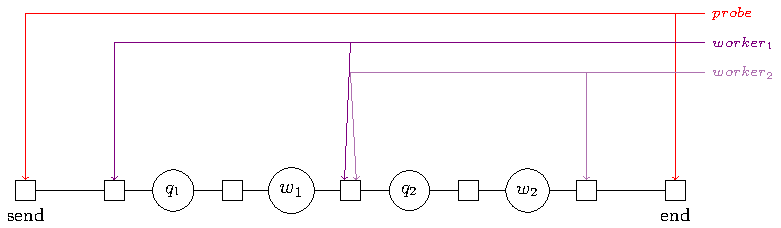
\includegraphics[scale=1.2, width=\textwidth]{tikz/mm1k.pdf} 
        \end{center}
        \caption{Outcome diagram of the system. The labeled coloured lines represent the probes that were inserted. $q_{1, 2}$ outcomes represent the queues. There the messages are forwarded to the workers. $w_{1,2}$ represent the workers whose task is doing $n$ loops. \\
        As we do not wish to observe the queues, but the whole behaviour of the worker components, we can insert probes from when the message is received to when the worker loops end.}
        \label{fig:mm1k}
    \end{figure}

    \subsection{Determining parameters dynamically}
        We stated previously that determining parameters is something that must be done with an underlying knowledge of the system (\cref{subsec:dMax}). The oscilloscope can provide knowledge of the system. \cref{fig:w1w2hb} shows an example of worker\_1 and worker\_2 as observed in the oscilloscope.

        The engineer supposes that the workers executions should take a maximum of 4 ms to complete, but doesn't actually know how long the executions should take. The engineer, after having set $dMax = 4ms$, observes the graph \cref{fig:w1w2hb} on the left in the oscilloscope.

    The oscilloscope shows the engineer that their assumptions do not correspond to the actual system $\Delta$Q. The user can then modify the parameters to observe the actual worker's behaviour. By setting $dMax$ to 8 ms, they can observe the worker's $\Delta$Qs failure approaching $0$ on the right Figure in \cref{fig:w1w2hb}.

    On the other hand, the engineer's assumption could have been what they truly expected from the system. In this case, the oscilloscope tells him that the system is not behaving as expected. 

\begin{figure}[H]
            \centering
            \begin{subfigure}{.5\textwidth}
                \centering
                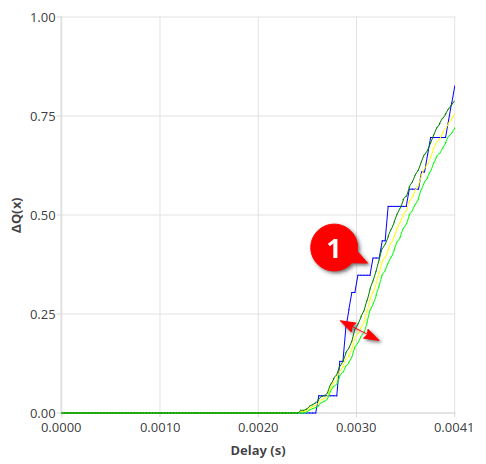
\includegraphics[width=0.98\textwidth]{img/overload_2/worker_1a.png}
                \label{fig:w14}
            \end{subfigure}%
            \begin{subfigure}{.5\textwidth}
                \centering
                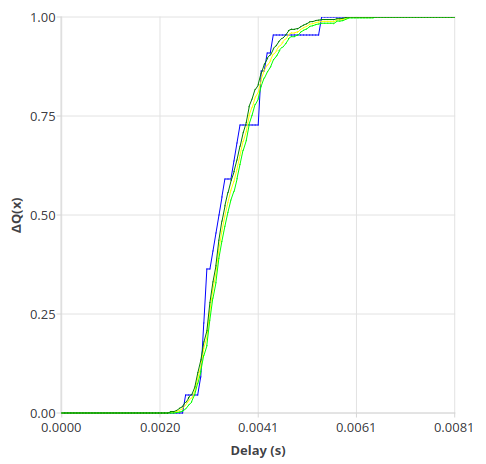
\includegraphics[width =0.98\textwidth]{img/overload_2/worker_1_8.png}
                \label{fig:w18}
            \end{subfigure}
            \caption{\textbf{Left}: worker\_1 $\Delta$Q with $dMax = 4ms$. (Green, between the arrow): Mean and confidence bounds of $\Delta$Qs in polling window. (1, blue): Observed $\Delta$Q in sampling window. The worker failure tends to 0.25. \\
            \textbf{Right}: worker\_1 $\Delta$Q with $dMax$ = 8ms. The worker failure now tends to 0. \\
            In both graphs we can observe how the observed $\Delta$Q of the sampling window is not precise. The step function representation of it fluctuates. The mean and confidence bounds provide a more precise representation of the $\Delta$Qs of worker\_1 over a polling window.}%
            \label{fig:w1w2hb}
            \end{figure}

    \subsubsection{Low Load} 
   We will send 50 messages per second to observe the system under test to get key properties. The workers do a million loops. \\
    We can observe in the left graph in \cref{fig:norm_ex} that the average worker's execution takes $\approx$ 33ms. We then have $\mu_{worker} = \frac{1}{0.0033 s} \approx 300$ req/s. Thus, $\rho = \frac{50}{300} = 0.1\overline{6}$, we can assume the system is at low load.

    At low load (\cref{fig:norm_ex}), the system is behaving \textbf{linearly}. Recall \cref{indep_hyp}, at low load the sum of the two delays will overlap with the observed total delay. We can observe in the oscilloscope the probe \textbf{observed $\Delta$Q} and \textbf{calculated $\Delta$Q} confidence bounds overlap. 
        \begin{figure}[H]
            \centering
            \begin{subfigure}{.5\textwidth}
                \centering
                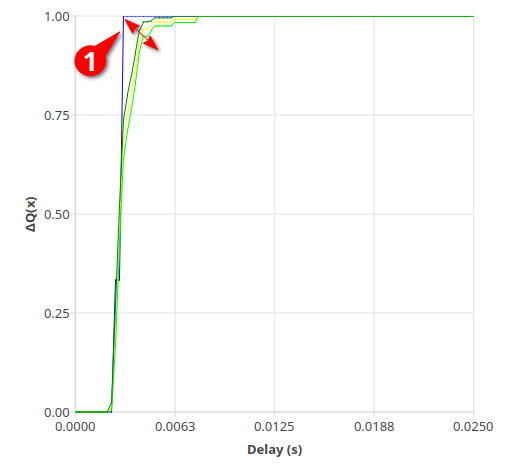
\includegraphics[width=0.98\textwidth]{img/overload_2/50_workeran.png}
                \label{fig:norm_ex_1}
            \end{subfigure}%
            \begin{subfigure}{.5\textwidth}
                \centering
                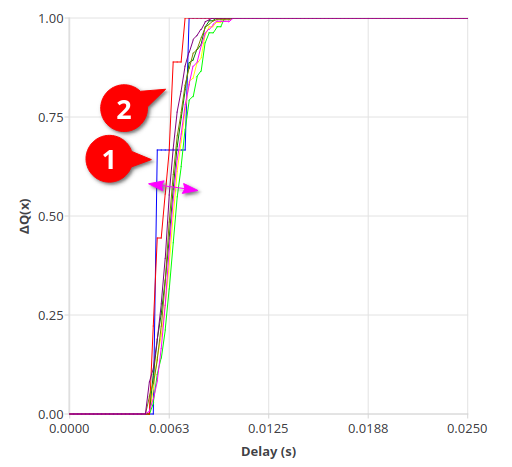
\includegraphics[width =0.98\textwidth]{img/overload_2/50_probe2.png}
                \label{fig:norm_ex_2}
            \end{subfigure}
            \caption{Graphs for $\lambda = 50$. Left: worker\_1 $\Delta$Qs. (1, Blue): The observed $\Delta$Q. (Green, between arrows): Observed polling window confidence bounds. \\
            Right: ``probe'' $\Delta$Qs. (1, blue): The sampling window observed $\Delta$Q. (2, red): The sampling window calculated $\Delta$Q. (Magenta, between arrows): the observed and calculated $\Delta$Qs confidence bounds overlapping.}
            \label{fig:norm_ex}
        \end{figure}
    
\subsubsection{Early signs of overload}
    
    At load = 0.5 the system should start showing dependent behaviour. We can observe what happens when $\lambda = 150 \rightarrow \rho = 0.5$.
    
    Recall \ref{fig:cdf_indep}, a non-linear system does not obey superposition. The sum of the delay of the workers will deviate from the overall delay of ``probe''. In \cref{fig:ovovv}, this is the case. \\
    We can start to observe early signs of dependency even at $\rho = 0.5$. The mean of the observed $\Delta$Q is deviating from the calculated one. At the 50th percentile the deviation is \textit{minimal}, around 0.4 ms. Nevertheless, the precision of the paradigm and the oscilloscope allows even for these minimal deviations to appear on the graphs, being able to recognise \textit{non-linearity} and \textit{early signs of overload}. \\
    The superposition principle is not respected anymore, there is apparent \textbf{non-linearity}, and the fact that $\Delta$Q can recognise non-linear behaviour with \textbf{0.4ms precision} is impressive. The oscilloscope is a powerful tool that can help assess dependent behaviour in running systems.
 
       \begin{figure}[H]
            \centering
            \begin{subfigure}{.5\textwidth}
                \centering
                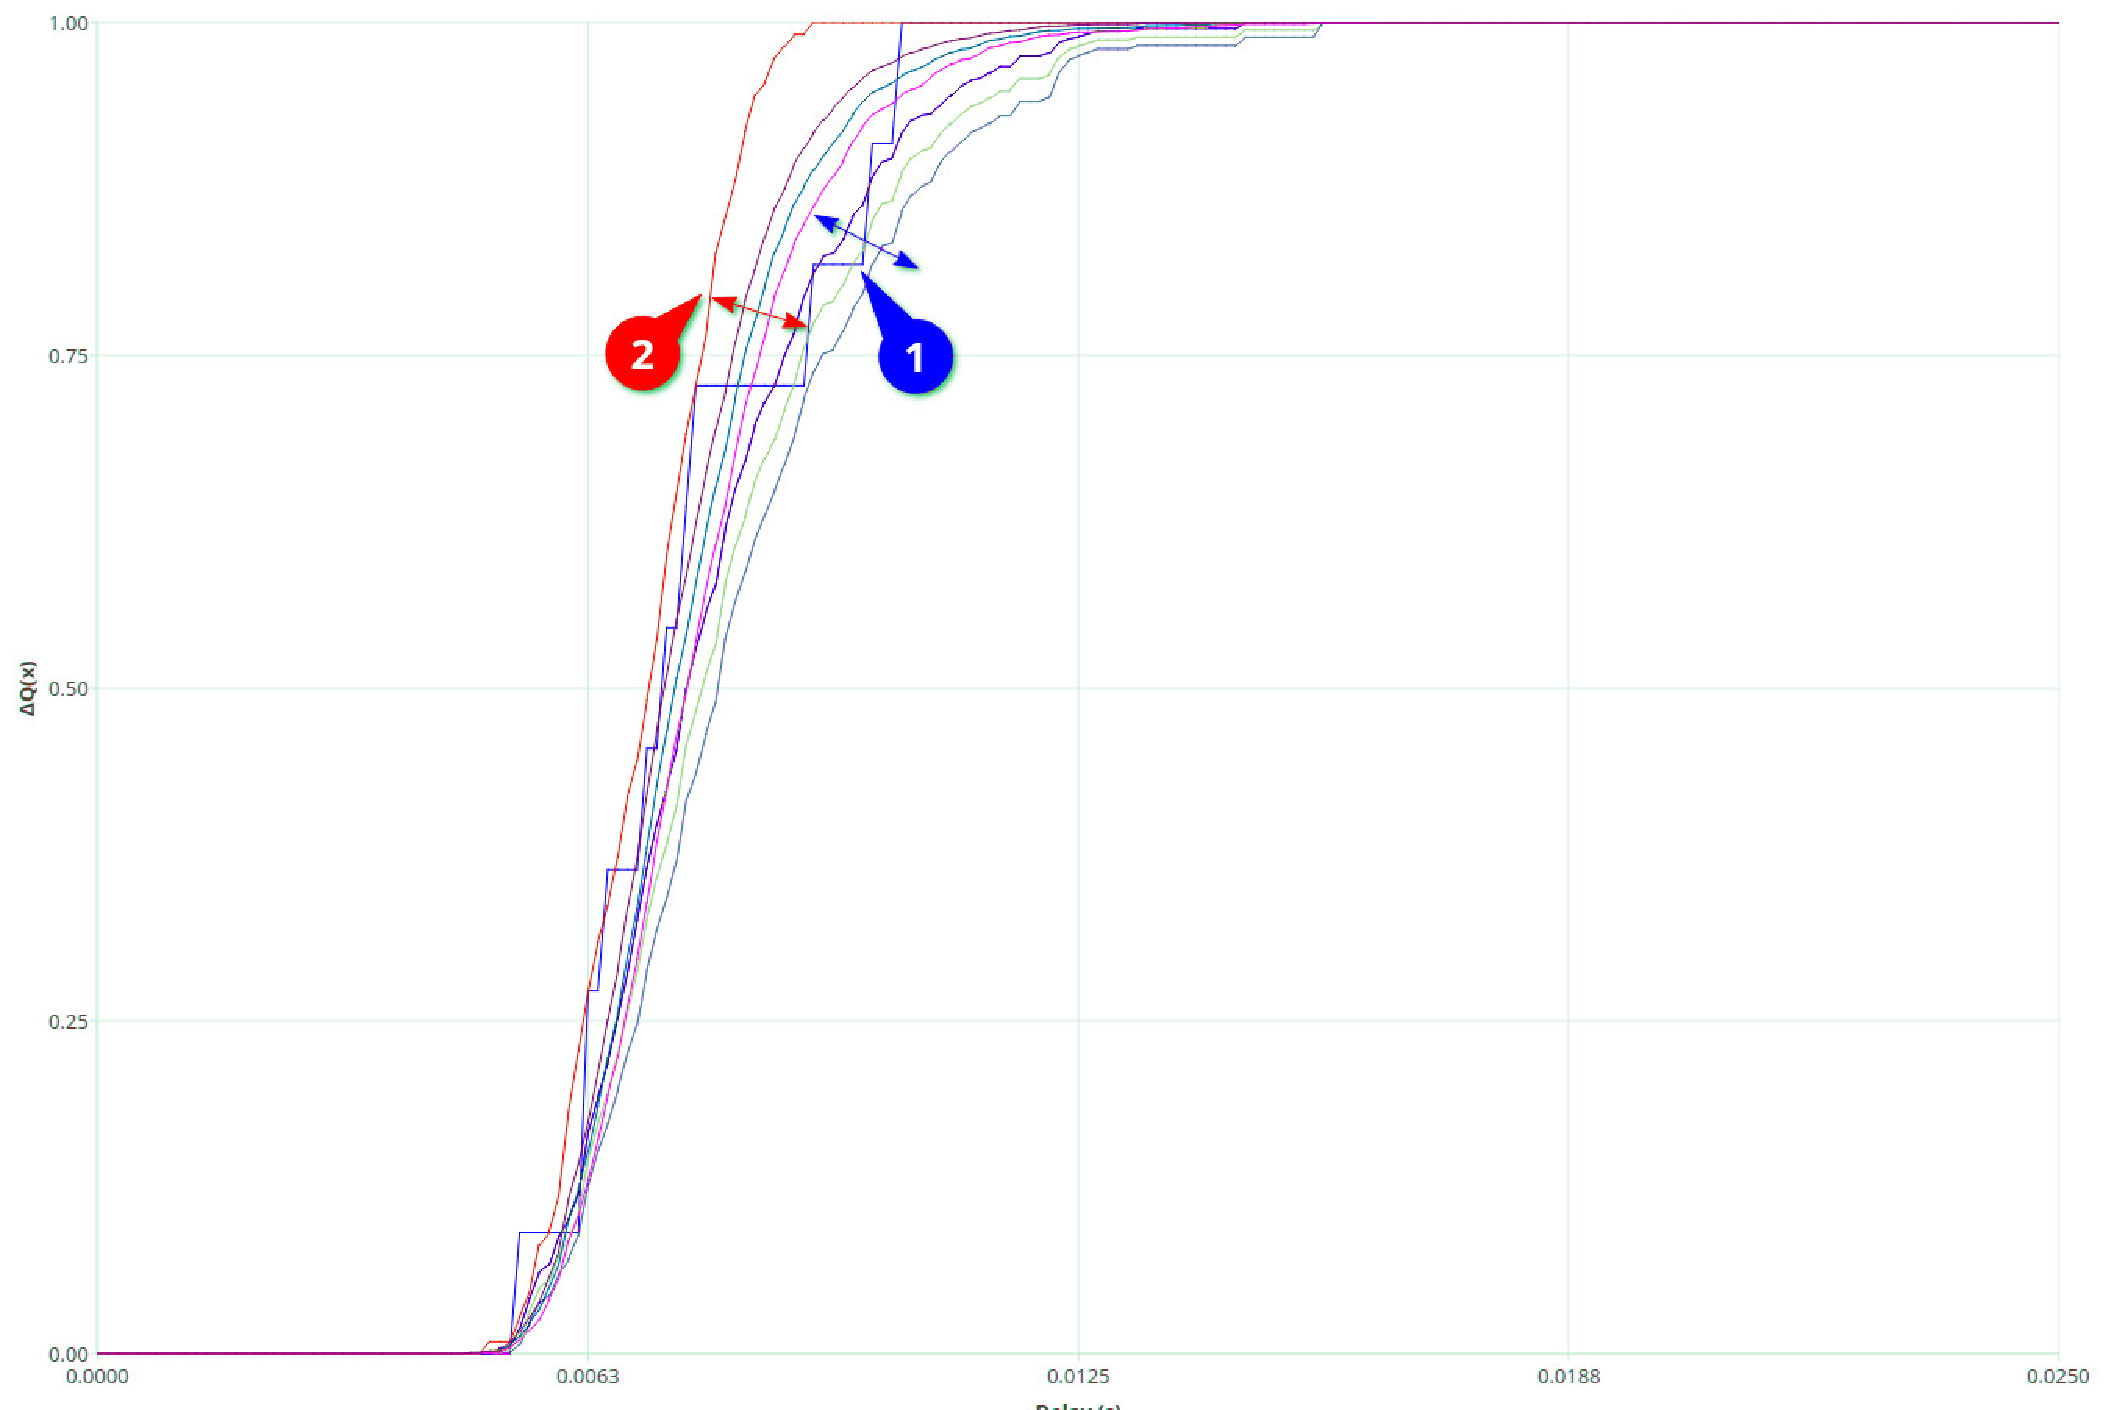
\includegraphics[width=0.98\textwidth]{img/overload_2/150_probe2.pdf}
                \label{fig:ovuvv}
            \end{subfigure}%
            \begin{subfigure}{.5\textwidth}
                \centering
                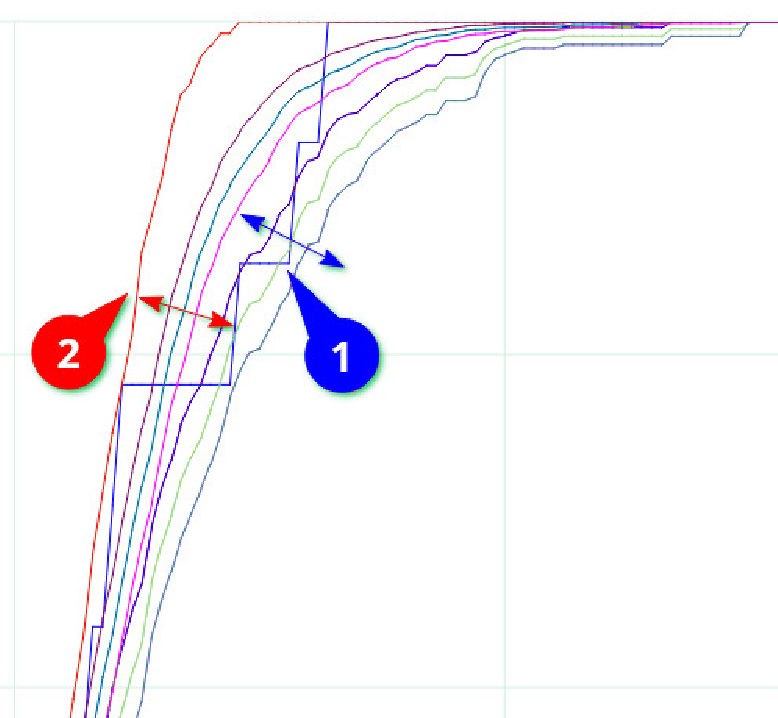
\includegraphics[width =0.98\textwidth]{img/overload_2/150_probe2zoom_cropped.pdf}
                \label{fig:ovovv}
            \end{subfigure}
            \caption{\textbf{Left}: The ``probe'' $\Delta$Qs as observed in a snapshot. \textbf{Right}: Zooming in the oscilloscope, we can observe a slight, but noticeable deviation. (1) Observed sampling window $\Delta$Q. (Arrow, blue, above): Its confidence bounds. (2) Calculated sampling window $\Delta$Q. (Arrow, red, below): Its confidence bounds. \\ The observed polling window confidence bounds are $>$ than the calculated $\Delta$Q bounds. The deviation at the median is of 0.4 ms, but it is noticeable in the oscilloscope.}
            \label{fig:avavv} 
        \end{figure}
       
\subsubsection{High load}
    Performance degradation at 0.5 offered load is already remarkable, the observed $\Delta$Qs and the calculated ones are slowly but surely deviating. The difference is seemingly minimal, but noticeable. We can go even further and observe the system under high load situations (\cref{fig:early_ov}). We set $\lambda = 250 \rightarrow \rho = 0.83$, just above the high load threshold.
    
       \begin{figure}[H]
            \centering
            \begin{subfigure}{.5\textwidth}
                \centering
                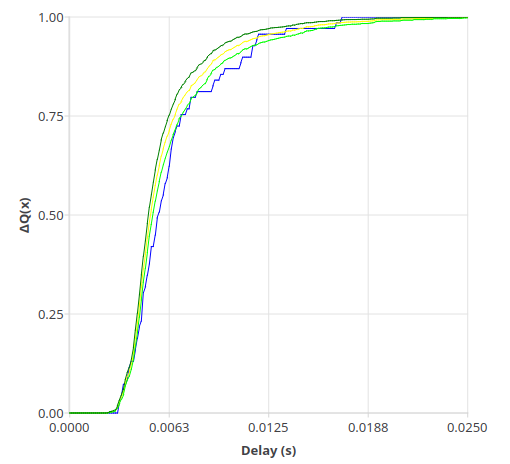
\includegraphics[width=0.98\textwidth]{img/overload_2/250_worker.png}
                \label{fig:high_load_1}
            \end{subfigure}%
            \begin{subfigure}{.5\textwidth}
                \centering
                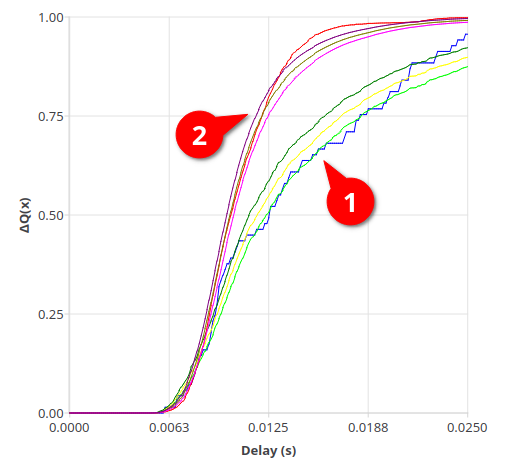
\includegraphics[width =0.98\textwidth]{img/overload_2/250_probe2.png}
                \label{fig:high_load_2}
            \end{subfigure}
            \caption{Graphs for $\lambda = 250$. \textbf{Left}: worker\_1 observed $\Delta$Q with its confidence bounds. \\
            \textbf{Right}: probe $\Delta$Q, in blue (1), the observed $\Delta$Q with its confidence bounds, in red (2) the calculated $\Delta$Q with its confidence bounds.}%
            \label{fig:early_ov}
        \end{figure} 
    This confirms what is expected by queueing theory, $\Delta$Q is capable of observing the basic observation requirements and capable of recognising dependency. While what is expected by the worker's observed $\Delta$Q is a nice normally distributed CDF with little to no failure. What we can observe on the probe is degraded performance in its observed $\Delta$Q mean. \\
    Due to dependency, high load and processor utilisation, the queue is filling up and the workers are taking more time to complete. If you recall \cref{fig:norm_ex}, the worker's delay distribution was less than the current one. We can see that it has completely degraded, with the average request taking almost double the time as under normal queueing conditions. 

    Further degradation can be observed by increasing $\lambda = {300, 350} \rightarrow \rho \ge 1$ (\cref{fig:hi_lo}).

    \begin{figure}[H]
            \centering
            \begin{subfigure}{.5\textwidth}
                \centering
                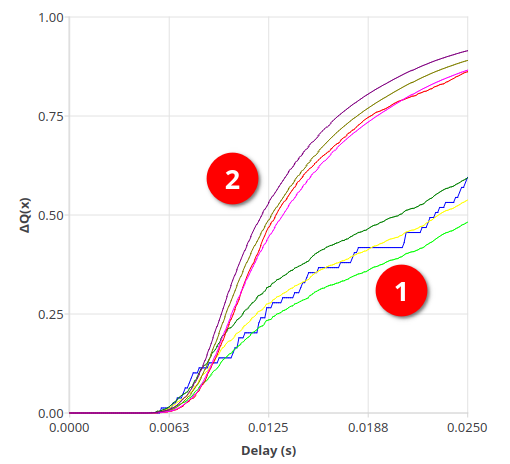
\includegraphics[width=0.98\textwidth]{img/overload_2/300_probe2.png}
                \label{fig:high_load_1}
            \end{subfigure}%
            \begin{subfigure}{.5\textwidth}
                \centering
                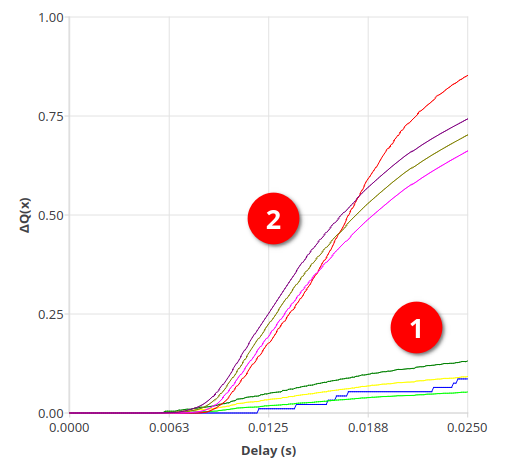
\includegraphics[width =0.98\textwidth]{img/overload_2/350_probe2.png}
                \label{fig:high_load_2}
            \end{subfigure}
            \caption{\textbf{Left}: (1) probe observed $\Delta$Q and confidence bounds for polling window. (2) probe calculated $\Delta$Q and confidence bounds for polling window at $\lambda = 300$. \textbf{Right}: probe $\Delta$Qs at $\lambda = 350$.}%
            \label{fig:hi_lo}%
        \end{figure}
    The system degrading is clear, the $\Delta$Qs show how almost all messages are being dropped or take $> dMax$. We can now look at triggers and how they can be useful to diagnose such cases.
  
    \subsubsection{Triggers}
        By observing the system under test in high load cases, we can set the load trigger by setting the sampling window to 1 second and trigger when outcome instances $\gtrapprox 150$. We can also set a trigger based on observation of the running system.

        \paragraph{QTA trigger}
            Recall the previous definition of $\Delta$Q (\cref{subsec:qta_i}), by observing the system, we create a QTA for the probe ``probe'' with: 25\% = 0.0075 s, 50\% = 0.0125 s, 75\% = 0.015s and minimum success rate = 0.9.

            By setting the trigger to fire for $\Delta$Q$_{obs} < QTA$. We captured a handful of snapshots. Here, $\lambda = 150$.
        
        \begin{figure}[H]
            \centering
            \begin{subfigure}{.5\textwidth}
                \centering
                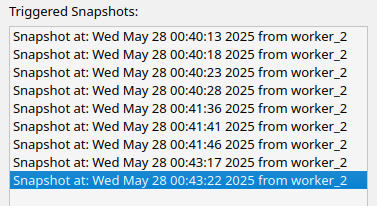
\includegraphics[width=0.98\textwidth]{img/overload_2/snapshots.png}
                \label{fig:high_load_1}
            \end{subfigure}%
            \begin{subfigure}{.5\textwidth}
                \centering
                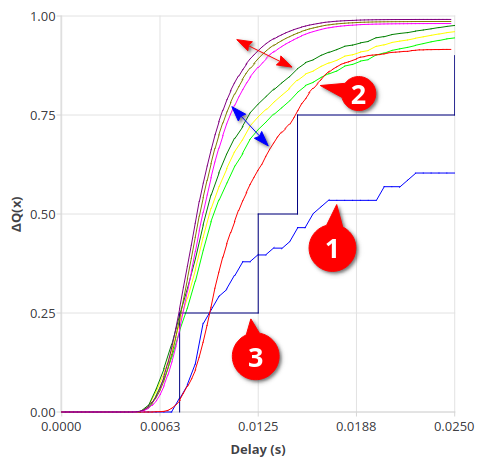
\includegraphics[width =0.98\textwidth]{img/overload_2/qta_triggerd2.png}
                \label{fig:high_load_2}
            \end{subfigure}
            \caption{\textbf{Left}: Snapshots for fired triggers. \\
            \textbf{Right}: (1) Observed $\Delta$Q in sampling window violating QTA (3). The confidence bounds for the observed polling window (blue, arrow, below) shows the system deteriorating. The calculated $\Delta$Q (2) is behaving worse than its confidence bounds (red, arrow, above). The system is overloaded, degrading and showing non-linear behaviour, this is captured by the QTA violation.} % 
            \label{fig:qta_viol_1}
        \end{figure}
        \paragraph{Instances trigger}

        QTA triggers can help detect non-linearity even before it becomes evident. \\
        By knowing the inner details of the system, setting a QTA on the number of instances can be useful. \cref{fig:qta_trig} is an example of a fired trigger on the number of instances.

        \begin{figure}[H]
            \begin{center}
                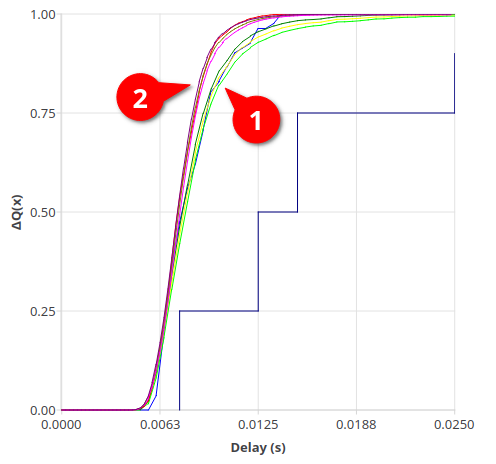
\includegraphics[scale=0.5]{img/overload_2/fired_samplea.png}
            \end{center}
            \caption{Graph of a snapshot for a fired trigger observing the load of a probe. (1) Observed $\Delta$Q confidence bounds. (2) Calculated $\Delta$Q confidence bounds. The trigger fires for observed load $> 150$ in a sampling window of 1 second. Even if the QTA requirement (step function) are not being violated, the system is showing early signs of non-linear behaviour.\\
            With knowledge about the system inner workings, smart triggers can be set on load to detect non-linear behaviour.}%
            \label{fig:qta_trig}%
        \end{figure}
        Even though the QTA requirement isn't being violated, the number of instances fires a trigger, where the user can observe that the system is showing early signs of overload.
  

    \section{Detecting slower workers in workers}
    \subsection{First to finish application}
        Next, we provide a synthetic application modeling an application that can be modeled by a first to finish operator

        \paragraph{Why first to finish?} Recall the previous FTF graph \cref{fig:ftf}. Assume a send request to "the cloud" that waits for a response or a timeout, it is modeled by a FTF operator. 
       \subsubsection{Using the wrong operator}
            What happens if the wrong operator is chosen to represent the causal relationships between the outcomes? What if the user believes that the system diagram is the one we presented before \cref{fig:mm1k}? The result on the oscilloscope will clearly show that something is wrong! 
            \begin{figure}[H]
                \centering
                \begin{subfigure}{.5\textwidth}
                    \centering
                    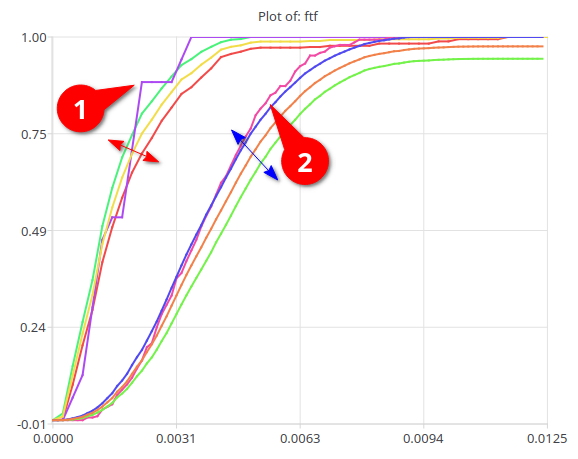
\includegraphics[width =0.98\textwidth]{img/bad1.png}
                    \label{fig:bad}
                \end{subfigure}%
                \begin{subfigure}{.5\textwidth}%
                    \centering%
                    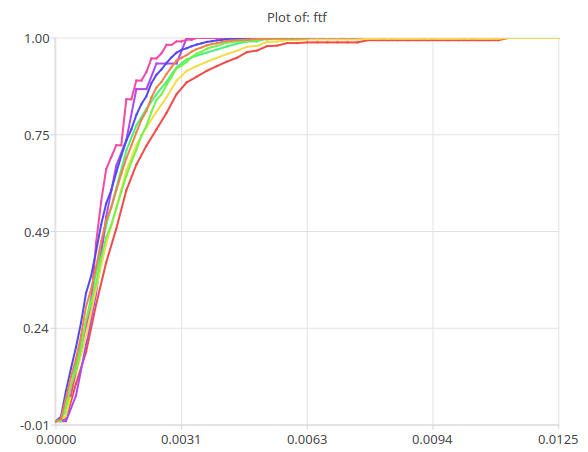
\includegraphics[width =0.98\textwidth]{img/good.png}%
                    \label{fig:good}%
                \end{subfigure}%
                \caption{\textit{(Left)} FTF plot \textbf{with wrong outcome diagram definition} as shown in the oscilloscope. (1) Observed $\Delta$Q. (2) Calculated $\Delta$Q. \\
                \textit{(Right)} FTF plot \textbf{with correct outcome diagram definition} as shown in the oscilloscope. Observed $\Delta$Q and calculated $\Delta$Q overlapping.}
                \label{fig:ftf_osc}%
            \end{figure}%
        On the left, we can observe how the \textbf{calculated $\Delta$Q} (2) is clearly greater than the \textbf{observed $\Delta$Q} (1). A difference this drastic tells us that the proposed outcome diagram does not correctly represent the actual system. On the right, if no dependencies are present and the correct operator is chosen, the two graphs will overlap.

        \subsubsection{Introducing a slower component}
            Let us introduce a slower worker into the system, we introduce an artificial delay into worker\_2 (about 20ms). If the oscilloscope works correctly, the paradigm operations are sound and no dependencies are present in the system, we should not see any difference in the observed and calculated $\Delta$Qs of the FTF operator.

            \begin{figure}[H]
                \centering 
                \begin{subfigure}{.5\textwidth}
                    \centering
                    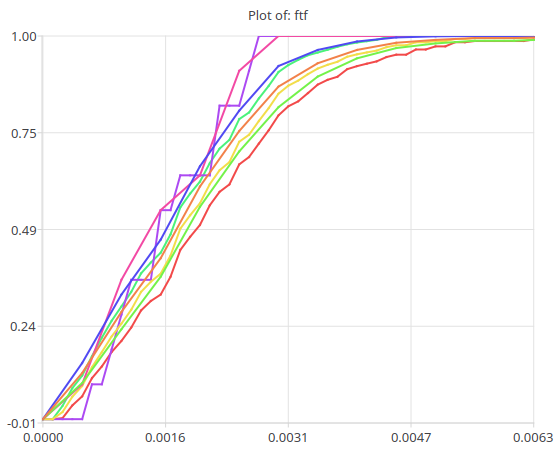
\includegraphics[width =0.98\textwidth]{img/delay31.png}
                    \label{fig:ftf_art_d}
                \end{subfigure}%
                \begin{subfigure}{.5\textwidth}%
                    \centering%
                    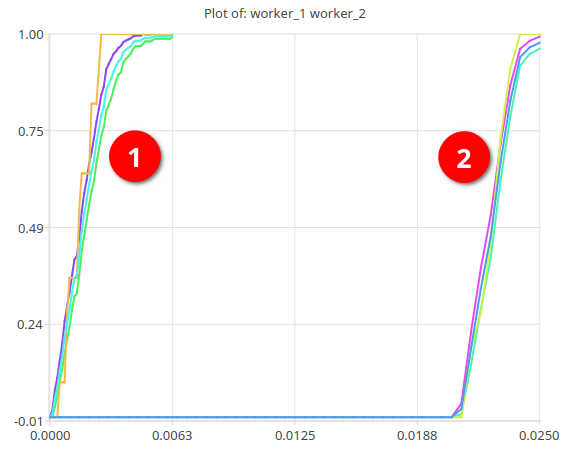
\includegraphics[width =0.98\textwidth]{img/delay32.png}%
                    \label{fig:ftf_art_dw}%
                \end{subfigure}%
                \caption{\textit{(Left)} FTF plot of worker\_1 and worker\_2, observed and calculated $\Delta$Q overlapping.\\
                \textit{(Right)} worker\_1 (1) and worker\_2 (2) $\Delta$Qs. \\
                The FTF plot correctly displays how worker\_2 does not have an effect on the ftf plot.}
                \label{fig:ftf_w1w2}%
            \end{figure}%


    \subsection{All to finish application}
    We can extend the previous application to an all-to-finish operator. This operator can for instance represent parallel work, a task that requires a lot of computation and can be done in separate pieces by separate workers. \cite{dq-tut}

        \subsubsection{Introducing a slower component}
            Like we did for the FTF operator, let's introduce a slower worker into the system. We introduce a slight delay to show how even a few milliseconds can be noticeable right away by a keen eye (or by triggers, which avoids having to look constantly at the graphs). Worker\_2 is 2ms slower.
 
            The difference in the worker's $\Delta$Q can be noticed with $\Delta \text{Q}_{w2} > \Delta \text{Q}_{w1}$ on the right in \cref{fig:slower_atf}. The difference can then be observed in the all-to-finish plot on the left in \cref{fig:slower_atf}, where the operator's $\Delta$Qs confidence bounds (both observed and calculated) can be overlaid on top of worker\_2 $\Delta$Q. This shows once again that the $\Delta$QSD algebraic foundation is sound. Moreover, the oscilloscope can be useful in detecting slower components in a system.

            \begin{figure}[H]
                \begin{center}
                    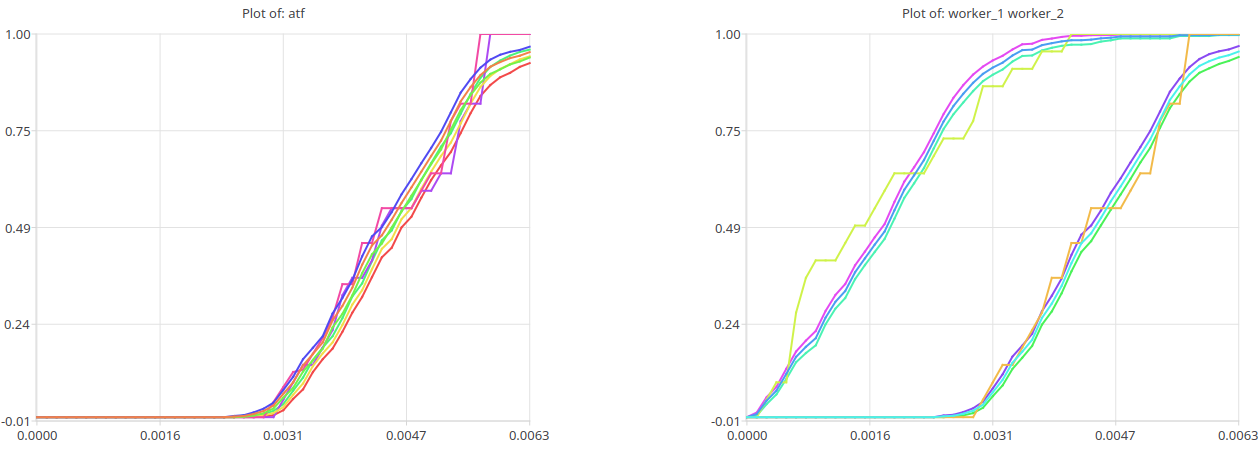
\includegraphics[scale = 0.5]{img/overload_2/w1w2atf.png}
                \end{center}
                \caption{\textbf{Left}: ATF plot with polling window confidence bounds for observed and calculated $\Delta$Q. \textbf{Right}: Worker's plots, worker\_2 is slower than worker\_1.}
                \label{fig:slower_atf}
            \end{figure}

    These plots show the usefulness of $\Delta$QSD, the system can be decomposed to understand which part of the system is showing hazards thanks to the notion of outcome diagrams. Furthermore, the causal relationships can be observed to determine the behaviour of a part down to the single component.


    \chapter{Performance study}
    \section{Convolution performance}
    We implemented two versions of the convolution algorithm as described before, the naïve version and the FFT version. We compared their performance when performing convolution on two $\Delta$Qs of equal bins.
    \begin{figure}[H]
        \begin{center}
            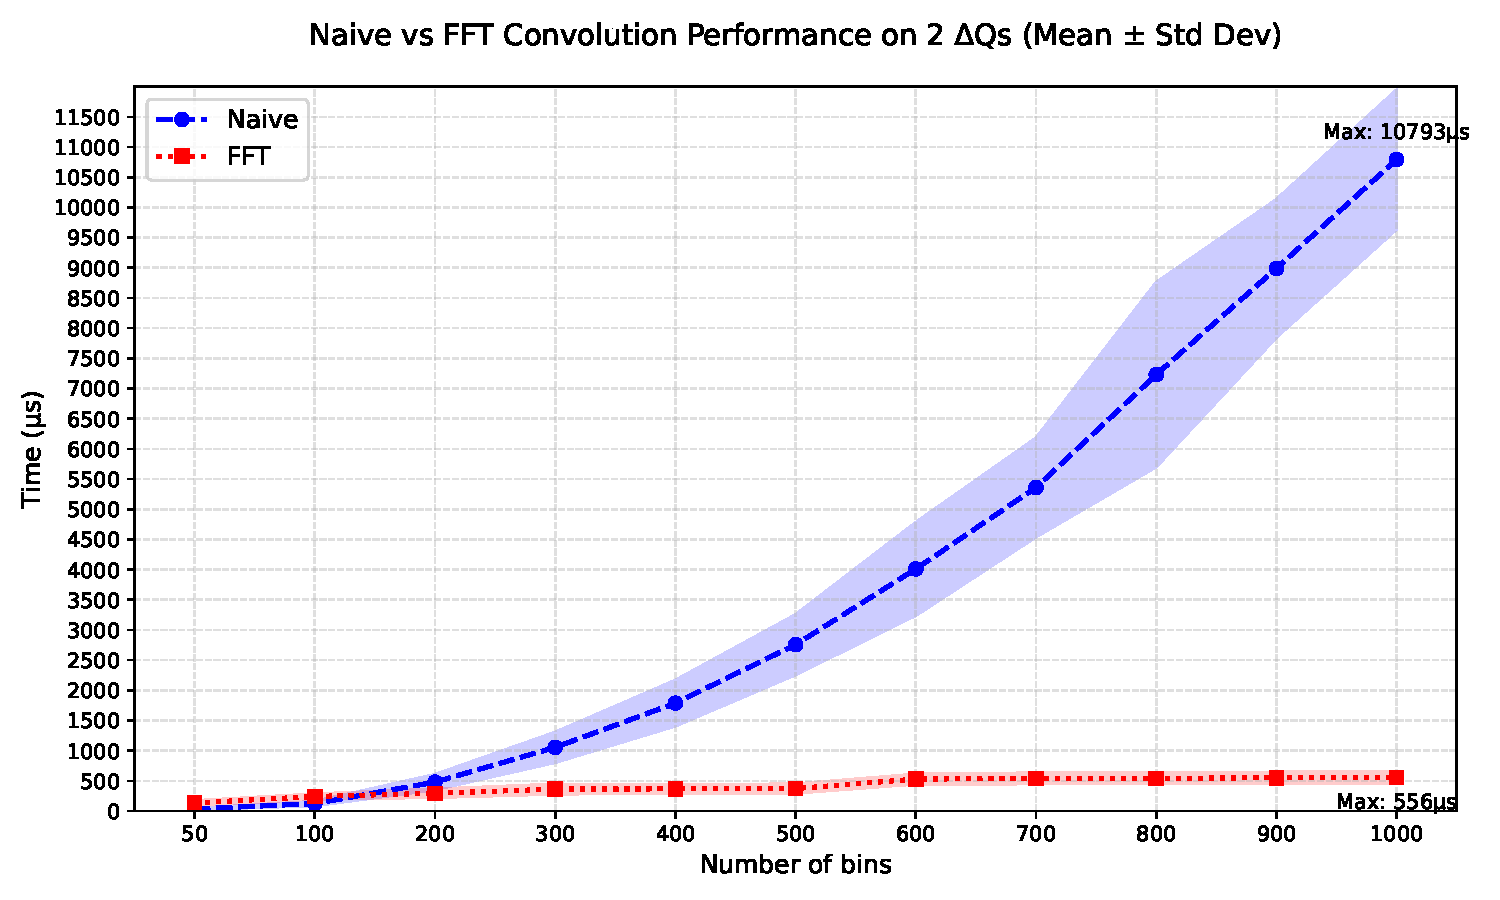
\includegraphics[width=0.85\textwidth]{img/conv_perf.pdf}
        \end{center}
        \caption{Performance comparison of two convolution algorithms}\label{fig:conv_perf}
    \end{figure}

    As expected, the naïve version has a time complexity of $\mathcal{O}(n^2)$ and quickly scales with the number of bins, this is clearly inefficient, as a more precise $\Delta$Q will result in a much slower program.


As for the FFT algorithm, it is slightly slower when the number of bins is lower than 100. This is due to the FFTW3 routine having slightly higher overhead.

    \section{Server performance}
    \section{Stub performance} 
     

    % Back cover page
    \medskip

    \printbibliography
        
    \appendix

    \chapter{Tests specifications}
    The tests were run on a laptop with the following specifications.
    \begin{itemize}
        \item \texttt{OS}: Manjaro Linux x86\_64, \texttt{Kernel:} 6.12.11-1-MANJARO
        \item \texttt{CPU}: Intel i5-6300U (4) @ 3.000GHz 
        \item \texttt{GPU}: Intel Skylake GT2 [HD Graphics 520]
        \item \texttt{RAM}: 16 GB DDR4 SDRAM—2133MHz
    \end{itemize}

\part{Addendum to Chapters 4 \& 5}
\chapter{Oscilloscope screenshots}

\section{System/Handle plots tab} \label{app:sidetab_ex}
    Here is a screenshot from the tab to create the system and handle plots (\cref{fig:sidetab_ex}).

    \begin{figure}[H]
        \begin{center}
            \includegraphics[scale = 0.6]{img/new_sys_cre.png}
        \end{center}
        \caption{System/Handle plots tab in oscilloscope.}
        \label{fig:sidetab_ex}
    \end{figure}

\newpage

\section{Parameters tab} \label{app:param_tab}
    Here is a screenshot of the parameters tab, with a set QTA showing up on a plot (\cref{fig:param_tab}).

    \begin{figure}[H]
        \begin{center}
            \includegraphics[width = \textwidth]{img/save_qta_manual.png}
        \end{center}
        \caption{Parameters tab in oscilloscope. The QTA set for worker\_1 can be seen on the plot.}
        \label{fig:param_tab}
    \end{figure}

\newpage

\section{Triggers tab} \label{app:trig_tab}
    Here is a screenshot of the triggers tab, with saved snapshots, QTA violation set for probe and a running plot (\cref{fig:triggers_tab}).

   \begin{figure}[H]
        \begin{center}
            \includegraphics[width = \textwidth]{img/manual/triggers.png}
        \end{center}
        \caption{Triggers tab in oscilloscope. The snapshots for the whole system are saved and can be observed.}
        \label{fig:triggers_tab}
    \end{figure}

\newpage

\section{Snapshot window} \label{app:snapshot}
    Here is a screenshot from the window observing a snapshot (\cref{fig:control_tab}).

    \begin{figure}[H]
        \begin{center}
            \includegraphics[width = \textwidth]{img/slow_g.png}
        \end{center}
        \caption{Snapshot window (above) over the running oscilloscope below.}
        \label{fig:control_tab} 
    \end{figure}

\newpage

\section{Connection controls} \label{app:con_control}
    Here is a screenshot of the available controls in the oscilloscope (\cref{fig:control_tab}).
   
   \begin{figure}[H]
        \begin{center}
            \includegraphics[width = \textwidth]{img/manual/server.png}
        \end{center}
        \caption{Connections control tab in the oscilloscope with the erlang and oscilloscope endpoints.}
        \label{fig:control_tab}
    \end{figure}

\newpage

\section{Widget view of GUI} \label{app:dash_wid}
    The GUI is composed of multiple building block, the widgets. The screenshot we provide here highlights the multiple widgets present in the GUI (\cref{fig:osc_widgs}). These widgets could be broken down into the multiple subwidgets that compose them.

    \begin{figure}[H]
        \begin{center}
            \includegraphics[width = \textwidth]{img/example_osc.png}
        \end{center}
        \caption{Widget view of the oscilloscope dashboard.}
        \label{fig:osc_widgs}
    \end{figure}



\part{User manual}
    \chapter{How to download and launch}
    To download the oscilloscope, go to the GitHub repository (\url{https://github.com/fnieri/DeltaQOscilloscope/}) and go to the releases page, there, you will find the different versions of the oscilloscope. For instruction purposes, we have made a pre-release to show where to find it.

   \begin{figure}[H]
        \begin{center}
            \includegraphics[width = \textwidth]{img/manual/releases.png}
        \end{center}
        \caption{Releases tab.}
    \end{figure}


   \begin{figure}[H]
        \begin{center}
            \includegraphics[width = \textwidth]{img/manual/release.png}
        \end{center}
        \caption{Sample release}
    \end{figure}

    The dq\_oscilloscope binary is the binary to download. By launching the binary on the CLI with:
    \begin{minted}{text}
        ./dq_oscilloscope
    \end{minted}
    The oscilliscope will launch.

    \chapter{Oscilloscope: How to use}
    \section{Establishing the adapter - oscilloscope connection}
    To connect to the oscilloscope to the server, you first need to start the oscilloscope server by setting the oscilloscope listening IP and port on the dashboard (\cref{fig:serv_endp}).

    \begin{figure}[H]
        \begin{center}
        \includegraphics[width = 0.8\textwidth]{img/manual/cserv.png}
        \end{center}
        \caption{Widget to set server endpoint in the oscilloscope}
        \label{fig:serv_endp}
    \end{figure}

    If the server cannot start, a popup will appear with the error.
    
    Once this is done, the adapter can establish a connection to the oscilloscope to send outcome instances (\cref{fig:est_con}). The adapter can now connect to the oscilloscope server.  
    
    \begin{figure}[H]
        \begin{center}
        \includegraphics[width = 0.8 \textwidth]{img/manual/connectadapter.png}
        \end{center}
        \caption{Establish connection from adapter to oscilloscope.}
        \label{fig:est_con}
    \end{figure}
    
    We now need to start the listener on the adapter (\cref{fig:est_list}).

     \begin{figure}[H]
        \begin{center}
        \includegraphics[width = 0.8 \textwidth]{img/manual/listener.png}
        \end{center}
         \caption{Adapter starting listener for commands and parameters from the oscilloscope}.
         \label{fig:est_list}
    \end{figure}

    If an error may arrive during the start-up of the listener, it will be printed out.

    Now, we can connect the oscilloscope to the adapter by setting the listener endpoint (\cref{fig:c_list}).
    
     \begin{figure}[H]
        \begin{center}
        \includegraphics[width = 0.8 \textwidth]{img/manual/endpoint.png}
        \end{center}
         \caption{Set Erlang listener endpoint in oscilloscope.}
         \label{fig:c_list}
    \end{figure}

    If the server cannot connect, an error will pop up. Once connected, the server can start and stop the adapter sending of the spans by clicking the two buttons below.

\section{Sidebar: Outcome diagram and plots}

    \subsection{Creating the system/outcome diagrams}

    You need to provide a textual description of your outcome diagram following the syntax which was defined previously.
    You can create your system by clicking on the \textbf{Create or edit system} button. If the parser successfully parsed the text, your system will be created and you can start setting the parameters for your probes.
    
    If the parser does not correctly parse the text, it will show a popup indicating the line where the error was produced and what it was expecting. 
    
    \subsection{Saving the system definition}

    The button \textbf{Save system to} gives you the possibility to save the textual definition of the outcome diagram to a file, you can save the file to any extension, but preferably the file will have the \textbf{.dq} extension.

    \subsection{Loading the system definition}

    The button \textbf{Load system to} gives you the possibility to load the textual definition of the outcome diagram you may have previously saved to a file, as for saving, you can load any file extension.

    
    \begin{figure}[H]
        \begin{center}
            \includegraphics[width = \textwidth]{img/save_system.png}
        \end{center}
    \end{figure}
        
\subsection{Managing the plots} 
    Once you have your system defined you can start adding plots of the $\Delta$Qs of the probes you inserted in your system.
    
    \subsubsection{Adding a plot}

    Multiple probes can be added at once in your plot, you can select the probes you want to add to a new plot by selecting them in the \textbf{"Add a new plot"} section. Then by clicking the \textbf{"Add plot"} button, the selected probes will be added to the plot.

\subsubsection{Editing a plot}
    You can remove the probes you have added to the plot by first clicking to it, this sets the plot as the \textbf{selected plot}. Once you have clicked the plot, a section will pop up beneath the rest of the controls on the sidebar. 
    
    In the section there are two subsections, one which shows the selected components which form the plot (those you have added previously), and the available components. You can select the probes you want to remove in the \textbf{"selected components"} zone, by clicking \textbf{"Remove selected components"} the components will be removed from the plot. Inversely, in the \textbf{"Available components"} section, you can select the plots you want to add, and by clicking \textbf{"Add selected components"} you can add the selected components to the selected plot.

\subsection{Removing a plot}
    By left-clicking the plot, a popup appears, you can click \textbf{"Remove plot"}, this removes it from the selected plot.



    \section{Sidebar: Probes settings}
    Now that you have create your outcome diagram, you can modify the probes settings to set the $dMax$ you want and the QTA you desire.

\subsection{Setting a QTA}
    You can set a QTA in the \textbf{"Set a QTA"} section, there you are presented with the possibility to:
    \begin{itemize}
        \item Select the probe for which you want to set the QTA.
        \item Set the QTA at the three percentiles (25\%, 50\%, 75\%), the text to the left indicates which percentile is which. You need to set the delay in seconds.
        \item The minimum amount of successful events you can allow, which is bigger than 75\%.
    \end{itemize}
    Of course, for the delay of the QTA at three percentiles, the delay at the percentile must be higher or equal than the delay at the previous percentile and higher than 0.
    
    By pressing \textit{"Save QTA settings"} you will save the QTA for the defined probe.

\subsection{Setting the parameters of a probe}
    You can set the parameters for a probe in its section.
    To the left you can select the probe you want to set the parameter for. 
    We provide a slider (which goes from -10 to 10) for the $n$ parameters, to the right of the slider, you can select the number of bins for the probe. The maximum delay calculated will be shown below.

    Once you press \textbf{"Save delay"}, a message to the erlang wrapper will be sent, which will set the maximum delay you have set in the wrapper.

    \begin{figure}[H]
        \begin{center}
            \includegraphics[width = \textwidth]{img/save_qta.png}
        \end{center}
        \caption{Probes settings tab. Above: QTA settings. Below: Probe parameters settings.}
    \end{figure}



    \section{Triggers}
    In the triggers section you can define which triggers to apply for a given probe, once selected, they will be automatically activated.

    Once a trigger is triggered, the oscilloscope will keep recording the system for a few seconds. Once stopped, under the "snapshots" section, you can click the snapshots to view them in a separate section, there, you can observe the $\Delta$Qs of all the probes before and after the trigger was triggered. You can discard the snapshot by left clicking on it and clicking \textit{"Delete snapshot"}.

     \begin{figure}[H]
        \begin{center}
        \includegraphics[width = \textwidth]{img/manual/triggers.png}
        \end{center}
        \caption{Examples of the QTA being set for a probe "probe". Once a trigger is fired, the resulting snapshot from the fired trigger will be available under "Triggered snapshots".}
    \end{figure}

\section{Snapshots}
    The snapshots can be observed to look at the state of the system, before, during and after the trigger has been fired.

    By clicking on the snapshot in the "triggered snapshots" section, a new window will popup where you can observe the system. A slider allows you to move backwards and forwards in time, observing the state of a probe in time.
 
    \begin{figure}[H]
        \begin{center}
        \includegraphics[width = \textwidth]{img/manual/snapshot.png}
        \end{center}
        \caption{Example of a snapshot, to the left, the graph at time $t$. To the right, the time of the graph on the left and a slider to advance backwards and forwards. As of right now, you can only select a probe at a time.}
    \end{figure}

    \section{Instrumenting the Erlang application}
    \subsection{Including the adapter}

    The Erlang project you need to instrument needs to include the adapter in its dependencies, to do that, you need to include it in your dependencies.

    \begin{minted}{text}
        %your_app.app.src
    {application, otel_getting_started, [
        ...
        {applications, [
            kernel,
            stdlib,
            opentelemetry,
            opentelemetry_api,
        opentelemetry_exporter,
        dqsd_otel
        ]},
        ...
        ]}.
    \end{minted}

    \begin{minted}{text}
    {deps, [
    {opentelemetry, "~> 1.3"},
    {opentelemetry_api, "~> 1.2"},
    {opentelemetry_exporter, "~> 1.0"},
    {dqsd_otel, {git, "https://github.com/fnieri/dqsd_otel.git", {tag, "the_latest_version_on_git"}}}
]}.
    \end{minted}
    
    Once you have the dependencies set up you can begin creating outcome instances for the oscilloscope.

    (\textbf{Note:} If the project were to change name, you can still find the project in https://github.com/fnieri/).

    \subsection{Starting spans}
        To start spans you need to call:
        \begin{minted}{erlang}
            {ProbeCtx, Pid} = dqsd_otel:start_span(<<"probe">>, #{attributes => [{attr, <<"my_attr_5o5s10">>}]}),
        \end{minted}
        This will give you the OpenTelemetry context of the probe and the Pid of the process to call upon end. It is left up to you to decide how to carry both in the execution.
        The function calls OpenTelemetry \texttt{?start\_span} macro, effectively replacing it.

    \subsection{Ending spans}
        To end spans you need to call:
        \begin{minted}{erlang}
            dqsd_otel:end_span(ProbeCtx, ProbePid)
        \end{minted}
        This will end the span on the OpenTelemetry side and end the outcome instance if it hasn't timedout
        The function calls OpenTelemetry \texttt{?end\_span} macro, effectively replacing it.

    \subsection{Failing outcome instances}
        To fail \textbf{custom} spans you need to call:
        \begin{minted}{erlang}
            dqsd_otel:fail_span(WorkerPid),
        \end{minted}
        Contrary to the other methods, this does not end OpenTelemetry spans, it is let up to you to decide how to handle failure in spans.

\section{Establishing connection to the oscilloscope}
    WIP

    
\part{Source Code Appendix}

\chapter{Grammar} \label{app:grammar}
This is the grammar for the ANTLR4 parser.
\lstinputlisting[style=mystyle, language=C++]{../RealTimeDeltaQSD/src/parser/DQGrammar.g4}

\chapter{C++ Source Files}

\section{Root folder}

\subsection{main.cpp}
This is the main file of the project.
\lstinputlisting[style=mystyle, language=C++]{../RealTimeDeltaQSD/src/main.cpp}

\subsection{Application.cpp}

This is a singleton that handles the global state of the application.
\lstinputlisting[style=mystyle, language=C++]{../RealTimeDeltaQSD/src/Application.cpp}


\section{Dashboard}
This folder contains the widgets that compose the dashboard.

\subsection{ColorRegistry.cpp} \label{code:coder}
\sloppy This class stores all the colors for all the QtSeries, moreover, it generates HSV colors based on the algorithm taken from \url{https://martin.ankerl.com/2009/12/09/how-to-create-random-colors-programmatically/}.
\lstinputlisting[style=mystyle, language=C++]{../RealTimeDeltaQSD/src/dashboard/ColorRegistry.cpp}

\subsection{CustomLegendEntry.cpp} \label{code:cle}
This class represents an entry in the plot legend.
\lstinputlisting[style=mystyle, language=C++]{../RealTimeDeltaQSD/src/dashboard/CustomLegendEntry.cpp}

\subsection{CustomLegendPanel.cpp} \label{code:clp}
This widget represents the legend panel for a plot, with entries corresponding to each series.
\lstinputlisting[style=mystyle, language=C++]{../RealTimeDeltaQSD/src/dashboard/CustomLegendPanel.cpp}

\subsection{DQPlotController.cpp} \label{code:dqpc}
This class is the controller of DeltaQPlot, based on the MVC design pattern.
\lstinputlisting[style=mystyle, language=C++]{../RealTimeDeltaQSD/src/dashboard/DQPlotController.cpp}

\subsection{DQPlotList.cpp} \label{code:dqpl}
This widget handles the adding and removing of probes series from a plot.
\lstinputlisting[style=mystyle, language=C++]{../RealTimeDeltaQSD/src/dashboard/DQPlotList.cpp}

\subsection{DelaySettingsWidget.cpp} \label{code:dsw}
This widget represent the slider widget to modify the parameters $dMax$, $\Delta$t and N.
\lstinputlisting[style=mystyle, language=C++]{../RealTimeDeltaQSD/src/dashboard/DelaySettingsWidget.cpp}

\subsection{DeltaQPlot.cpp} \label{code:dqp}
This widget is the widget containing a plot and its legend.
\lstinputlisting[style=mystyle, language=C++]{../RealTimeDeltaQSD/src/dashboard/DeltaQPlot.cpp}

\subsection{MainWindow.cpp} \label{code:mw}
This widget is the main window of the application, it has a tab to the side where the widgets to control the oscilloscope are. To the left, the panel where all plots are shown.
\lstinputlisting[style=mystyle, language=C++]{../RealTimeDeltaQSD/src/dashboard/MainWindow.cpp}

\subsection{NewPlotList.cpp} \label{code:npl}
This widget is the widget to add a new plot to the plots panel.
\lstinputlisting[style=mystyle, language=C++]{../RealTimeDeltaQSD/src/dashboard/NewPlotList.cpp}

\subsection{ObservableSettings.cpp} \label{code:os}
This widget is a tab that contains the settings for the probes (Setting a QTA, setting $dMax$).
\lstinputlisting[style=mystyle, language=C++]{../RealTimeDeltaQSD/src/dashboard/ObservableSettings.cpp}

\subsection{SamplingRateWidget.cpp} \label{code:srw}
This widget allows the sampling rate to be changed via a slider.
\lstinputlisting[style=mystyle, language=C++]{../RealTimeDeltaQSD/src/dashboard/SamplingRateWidget.cpp}

\subsection{QTAInputWidget.cpp} \label{code:qiw}
This widget allows the QTA to be set for a probe
\lstinputlisting[style=mystyle, language=C++]{../RealTimeDeltaQSD/src/dashboard/QTAInputWidget.cpp}

\subsection{Sidebar.cpp} \label{code:side}
This widget is a tab where the user can handle the system, add/remove plots and change the sampling rate.
\lstinputlisting[style=mystyle, language=C++]{../RealTimeDeltaQSD/src/dashboard/Sidebar.cpp}

\subsection{SnapshotViewerWindow.cpp} \label{code:svw}
This is a window to observe a snapshot from the triggers tab.
\lstinputlisting[style=mystyle, language=C++]{../RealTimeDeltaQSD/src/dashboard/SnapshotViewerWindow.cpp}

\subsection{StubControlWidget.cpp} \label{code:scw}
This widget allows to open the server on the IP and Port defined by the user and to connect to the adapter on the IP and port specified by the user.
\lstinputlisting[style=mystyle, language=C++]{../RealTimeDeltaQSD/src/dashboard/StubControlWidget.cpp}

\subsection{SystemCreationWidget.cpp} \label{code:syscw}
This widget allows the creation/update of a system, loading an already existing one or saving one.
\lstinputlisting[style=mystyle, language=C++]{../RealTimeDeltaQSD/src/dashboard/SystemCreationWidget.cpp}

\subsection{TriggersTab.cpp} \label{code:tt}
This tab holds the widgets to set/remove triggers and view fired ones. 
\lstinputlisting[style=mystyle, language=C++]{../RealTimeDeltaQSD/src/dashboard/TriggersTab.cpp}

\section{Outcome diagram}

The "diagram" folder contains everything related to outcome diagrams. Due to time related issues, there are some issues with the names. We will explain what each class represents, but it differs from the definitions which are explained in the thesis

\subsection{Observable.cpp} \label{code:obs}
The observable class represents a generic "observable" element of the outcome diagram, it is the base class for probes, outcome and operators. In this class one can calculate the observed $\Delta$Q, store the outcome instances (samples), set the parameters, set a QTA, add/remove triggers and get a snapshot. It is what we described throughout the whole paper as a probe.

\lstinputlisting[style=mystyle, language=C++]{../RealTimeDeltaQSD/src/diagram/Observable.cpp}
\subsection{Operator.cpp} \label{code:op}
This class represent a generic operator, it can be either a FTF, ATF or PC. It allows calculating the "calculated $\Delta$Q".
\lstinputlisting[style=mystyle, language=C++]{../RealTimeDeltaQSD/src/diagram/Operator.cpp}

\subsection{Outcome.cpp} \label{code:outc}
This class represents a simple outcome.
\lstinputlisting[style=mystyle, language=C++]{../RealTimeDeltaQSD/src/diagram/Outcome.cpp}

\subsection{Probe.cpp} \label{code:probe}
This class represents what we described as "sub-outcome diagram". As the operator class, it allows calculating the "calculated $\Delta$Q".
\lstinputlisting[style=mystyle, language=C++]{../RealTimeDeltaQSD/src/diagram/Probe.cpp}

\subsection{System.cpp} \label{code:sys}
This class represents the system, the whole outcome diagram. It coordinates the various parts of the outcome diagram.
\lstinputlisting[style=mystyle, language=C++]{../RealTimeDeltaQSD/src/diagram/System.cpp}

\section{$\Delta$Q (maths)}
The "maths" folder represents all the classes related to $\Delta$Q, where mathematical operations are being done (hence the "maths" name).

\subsection{ConfidenceInterval.cpp} \label{code:ci}
This class represents the confidence bounds described earlier.
\lstinputlisting[style=mystyle, language=C++]{../RealTimeDeltaQSD/src/maths/ConfidenceInterval.cpp}

\subsection{DeltaQ.cpp} \label{code:dq}
This class represents a $\Delta$Q. It supports calculating a $\Delta$Q given multiple samples, calculating the quartiles of a $\Delta$Q, it supports various arithmetical transformations.
\lstinputlisting[style=mystyle, language=C++]{../RealTimeDeltaQSD/src/maths/DeltaQ.cpp}

\subsection{DeltaQOperations.cpp} \label{code:dqop}
This file contains the definition of all the operations that can be done on a $\Delta$Q or on $\Delta$Qs, specified in the implementation chapter. Convolution (naive, FFT), FTF, ATF, PC operators, rebinning.
\lstinputlisting[style=mystyle, language=C++]{../RealTimeDeltaQSD/src/maths/DeltaQOperations.cpp}

\subsection{Snapshot.cpp} \label{code:snaps}
This class represents a single snapshot of a probe. It contains the QTA, observable $\Delta$Q and calculated $\Delta$Q at time t.
\lstinputlisting[style=mystyle, language=C++]{../RealTimeDeltaQSD/src/maths/Snapshot.cpp}

\subsection{TriggerManager.cpp} \label{code:trigman}
This class is the manager of triggers for a probe. It can add/remove/evaluate triggers.
\lstinputlisting[style=mystyle, language=C++]{../RealTimeDeltaQSD/src/maths/TriggerManager.cpp}

\subsection{Triggers.cpp} \label{code:trigg}
This class contains the conditions of the triggers selected by the user. The trigger manager evaluates the conditions at runtime. The Actions namespace is WIP.
\lstinputlisting[style=mystyle, language=C++]{../RealTimeDeltaQSD/src/maths/Triggers.cpp}

\section{parser}

\subsection{SystemBuilder.cpp} \label{code:sysb}
This class builds a new outcome diagram (system class) given an AST biult when parsing.
\lstinputlisting[style=mystyle, language=C++]{../RealTimeDeltaQSD/src/parser/SystemBuilder.cpp}

\subsection{SystemParserInterface.cpp} \label{code:syspi}
This class is an interface to be called by the dashboard to avoid communicating directly to ANTLR. It throws errors which are caught by the caller if the parsing was unsuccessful.
\lstinputlisting[style=mystyle, language=C++]{../RealTimeDeltaQSD/src/parser/SystemParserInterface.cpp}

\section{server}

\subsection{Server.cpp} \label{code:serv}
This class represents the server which receives and sends messages from Erlang.
\lstinputlisting[style=mystyle, language=C++]{../RealTimeDeltaQSD/src/server/Server.cpp}

\chapter{C++ Header Files}

\section{Root}

\subsection{Application.h}
\lstinputlisting[style=mystyle, language=C++]{../RealTimeDeltaQSD/src/Application.h}

\section{dashboard}

\subsection{ColorRegistry.h}
\lstinputlisting[style=mystyle, language=C++]{../RealTimeDeltaQSD/src/dashboard/ColorRegistry.h}

\subsection{CustomLegendEntry.h}
\lstinputlisting[style=mystyle, language=C++]{../RealTimeDeltaQSD/src/dashboard/CustomLegendEntry.h}

\subsection{CustomLegendPanel.h}
\lstinputlisting[style=mystyle, language=C++]{../RealTimeDeltaQSD/src/dashboard/CustomLegendPanel.h}

\subsection{DQPlotController.h}
\lstinputlisting[style=mystyle, language=C++]{../RealTimeDeltaQSD/src/dashboard/DQPlotController.h}

\subsection{DQPlotList.h}
\lstinputlisting[style=mystyle, language=C++]{../RealTimeDeltaQSD/src/dashboard/DQPlotList.h}

\subsection{DelaySettingsWidget.h}
\lstinputlisting[style=mystyle, language=C++]{../RealTimeDeltaQSD/src/dashboard/DelaySettingsWidget.h}

\subsection{DeltaQPlot.h}
\lstinputlisting[style=mystyle, language=C++]{../RealTimeDeltaQSD/src/dashboard/DeltaQPlot.h}

\subsection{MainWindow.h}
\lstinputlisting[style=mystyle, language=C++]{../RealTimeDeltaQSD/src/dashboard/MainWindow.h}

\subsection{NewPlotList.h}
\lstinputlisting[style=mystyle, language=C++]{../RealTimeDeltaQSD/src/dashboard/NewPlotList.h}

\subsection{ObservableSettings.h}
\lstinputlisting[style=mystyle, language=C++]{../RealTimeDeltaQSD/src/dashboard/ObservableSettings.h}

\subsection{SamplingRateWidget.h}
\lstinputlisting[style=mystyle, language=C++]{../RealTimeDeltaQSD/src/dashboard/SamplingRateWidget.h}

\subsection{QTAInputWidget.h}
\lstinputlisting[style=mystyle, language=C++]{../RealTimeDeltaQSD/src/dashboard/QTAInputWidget.h}

\subsection{Sidebar.h}
\lstinputlisting[style=mystyle, language=C++]{../RealTimeDeltaQSD/src/dashboard/Sidebar.h}

\subsection{SnapshotViewerWindow.h}
\lstinputlisting[style=mystyle, language=C++]{../RealTimeDeltaQSD/src/dashboard/SnapshotViewerWindow.h}

\subsection{StubControlWidget.h}
\lstinputlisting[style=mystyle, language=C++]{../RealTimeDeltaQSD/src/dashboard/StubControlWidget.h}

\subsection{SystemCreationWidget.h}
\lstinputlisting[style=mystyle, language=C++]{../RealTimeDeltaQSD/src/dashboard/SystemCreationWidget.h}

\subsection{TriggersTab.h}
\lstinputlisting[style=mystyle, language=C++]{../RealTimeDeltaQSD/src/dashboard/TriggersTab.h}

\section{diagram}

\subsection{Observable.h}
\lstinputlisting[style=mystyle, language=C++]{../RealTimeDeltaQSD/src/diagram/Observable.h}

\subsection{Operator.h}
\lstinputlisting[style=mystyle, language=C++]{../RealTimeDeltaQSD/src/diagram/Operator.h}

\subsection{OperatorType.h}
\lstinputlisting[style=mystyle, language=C++]{../RealTimeDeltaQSD/src/diagram/OperatorType.h}

\subsection{Outcome.h}
\lstinputlisting[style=mystyle, language=C++]{../RealTimeDeltaQSD/src/diagram/Outcome.h}

\subsection{Probe.h}
\lstinputlisting[style=mystyle, language=C++]{../RealTimeDeltaQSD/src/diagram/Probe.h}

\subsection{Sample.h}
This struct represents an outcome instance.
\lstinputlisting[style=mystyle, language=C++]{../RealTimeDeltaQSD/src/diagram/Sample.h}

\subsection{System.h}
\lstinputlisting[style=mystyle, language=C++]{../RealTimeDeltaQSD/src/diagram/System.h}

\section{$\Delta$Q (maths)}

\subsection{ConfidenceInterval.h}
\lstinputlisting[style=mystyle, language=C++]{../RealTimeDeltaQSD/src/maths/ConfidenceInterval.h}

\subsection{DeltaQ.h}
\lstinputlisting[style=mystyle, language=C++]{../RealTimeDeltaQSD/src/maths/DeltaQ.h}

\subsection{DeltaQOperations.h}
\lstinputlisting[style=mystyle, language=C++]{../RealTimeDeltaQSD/src/maths/DeltaQOperations.h}

\subsection{DeltaQRepr.h}
\lstinputlisting[style=mystyle, language=C++]{../RealTimeDeltaQSD/src/maths/DeltaQRepr.h}

\subsection{QTA.h}
This class represent a sample QTA.
\lstinputlisting[style=mystyle, language=C++]{../RealTimeDeltaQSD/src/maths/QTA.h}

\subsection{Snapshot.h}
\lstinputlisting[style=mystyle, language=C++]{../RealTimeDeltaQSD/src/maths/Snapshot.h}

\subsection{TriggerManager.h}
\lstinputlisting[style=mystyle, language=C++]{../RealTimeDeltaQSD/src/maths/TriggerManager.h}

\subsection{TriggerTypes.h}
\lstinputlisting[style=mystyle, language=C++]{../RealTimeDeltaQSD/src/maths/TriggerTypes.h}

\subsection{Triggers.h}
\lstinputlisting[style=mystyle, language=C++]{../RealTimeDeltaQSD/src/maths/Triggers.h}

\section{parser}

\subsection{SystemBuilder.h}
\lstinputlisting[style=mystyle, language=C++]{../RealTimeDeltaQSD/src/parser/SystemBuilder.h}

\subsection{SystemErrorListener.h}
\lstinputlisting[style=mystyle, language=C++]{../RealTimeDeltaQSD/src/parser/SystemErrorListener.h}

\subsection{SystemParserInterface.h}
\lstinputlisting[style=mystyle, language=C++]{../RealTimeDeltaQSD/src/parser/SystemParserInterface.h}

\section{server}

\subsection{Server.h}
\lstinputlisting[style=mystyle, language=C++]{../RealTimeDeltaQSD/src/server/Server.h}

\chapter{Build Configuration Files}

\section{src/CMakeLists.txt}
\lstinputlisting[style=mystyle, ]{../RealTimeDeltaQSD/src/CMakeLists.txt}

\section{dashboard/CMakeLists.txt}
\lstinputlisting[style=mystyle, ]{../RealTimeDeltaQSD/src/dashboard/CMakeLists.txt}

\section{diagram/CMakeLists.txt}
\lstinputlisting[style=mystyle, ]{../RealTimeDeltaQSD/src/diagram/CMakeLists.txt}

\section{maths/CMakeLists.txt}
\lstinputlisting[style=mystyle, ]{../RealTimeDeltaQSD/src/maths/CMakeLists.txt}

\section{parser/CMakeLists.txt}
\lstinputlisting[style=mystyle, ]{../RealTimeDeltaQSD/src/parser/CMakeLists.txt}

\section{server/CMakeLists.txt}
\lstinputlisting[style=mystyle, ]{../RealTimeDeltaQSD/src/server/CMakeLists.txt}

\chapter{Erlang Source Files}

\section{Root}

\subsection{dqsd\_otel.erl}
The $\Delta$Q adapter, it can start, fail, end spans and start and end with\_spans, communicates to the TCP client to send outcome instances to the oscilloscope.
\lstinputlisting[style=mystyle, language=erlang]{../dqsd_otel/src/dqsd_otel.erl}

\subsection{dqsd\_otel\_app.erl}
\lstinputlisting[style=mystyle, language=erlang]{../dqsd_otel/src/dqsd_otel_app.erl}

\subsection{dqsd\_otel\_sup.erl}
The supervisor of the adapter. It start the TCP server, client and adapter.
\lstinputlisting[style=mystyle, language=erlang]{../dqsd_otel/src/dqsd_otel_sup.erl}

\subsection{dqsd\_otel\_tcp\_client.erl}
The TCP client, it can send outcome instances to the oscilloscope.
\lstinputlisting[style=mystyle, language=erlang]{../dqsd_otel/src/dqsd_otel_tcp_client.erl}

\subsection{dqsd\_otel\_tcp\_server.erl}
The TCP server accepts messages from the oscilloscope and forwards them to the adapter to set the various settings.
\lstinputlisting[style=mystyle, language=erlang]{../dqsd_otel/src/dqsd_otel_tcp_server.erl}

\chapter{Erlang Application Files}

\section{Root}

\subsection{dqsd\_otel.app.src}
The app.src file of the adapter.
\lstinputlisting[style=mystyle, language=erlang]{../dqsd_otel/src/dqsd_otel.app.src}



    \backcoverpage


\end{document}
